\chapter{Model} \label{chapter-model}
% \epigraph{One of the very important components in the urban and agricultural land use model is the so-called \gls{bid-rent curve}. Regional and urban economists, city planners, and economic geographers have used this curve extensively as an analytical device.}{Yeung-Nan Shieh\cite{shiehWilhelmLaunhardtBidRent2004}}

% COULD CALL THIS THEORETICAL DEVELOPMENT OF THE MODEL AND MAKE A SEPERATE IMPLEMENTATION CHAPTER

This chapter links (**E USE A MORE SPECIFIC WORD THAN LINKS) % #E BUILD A PCITURE OF HOW THE MODEL DRAWS THESE TOGETHER... LIKE IT TAKES THESE THREAD (LIST THEM) AND COMBINES THEM INTO A MODEL THAT EXPLORE... USE THIS PARRARAPH TO DESCRIBE THE EXACT INTERCONNECTIONS

the theoretical discussions of the previous chapters with an agent-based simulation model. 

At the heart of the model is a real estate market in which owners, tenants, new entrants to the city and non-resident investors participate. We need to specify the market process in more detail. (???) % i DONT UNDERSTAND IF YOU ARE SAYING YOU NEED THIS? THE MODEL FILLS THIS GAP?? OR THIS IS AFILLER SENTECEN??? 
To do that we build up our model in a series of steps beginning with a notion of economic value, adding potential speculative gains, and finally describing a transaction process. 

\section{The general structure of the model}
The main goal of this research as been to add a financial system to the simple Alonzo model in order to examine the impact of financial cycles on urban productivity and distribution. The \gls{agent-based model} we develop has three major components: 

\begin{enumerate}
\item We incorporate the spatial structure of the city and its transportation system using a version of the \gls{bid-rent function} that drives all Alonzo-style models. This equation is embedded in the decision of every agent.

\item We incorporate the fundamental wealth production process of the city by using an \gls{urban scaling} law that captures Jacobs-style agglomeration effects. This allows us to bypass the complexities of labour and goods market adjustments and deal with the underlying long-term relationship between city  population and production. We have called the combination of this Jacob agglomeration effect with the Alonzo model an \gls{Alonzo-Jacobs model}.  Two difference equations operating on two aggregate variables incorporate the major insight of a half-century of \gls{neoclassical growth theory}.

\item To link the Alonzo-Jacobs model to the financial system, we develop an \gls{overlapping generations} model of the housing market with borrowers and lenders that tracks ownership and wealth. This turns out to be the most detailed and computationally-intensive part of the model.
\end{enumerate}

To recapitulate, we have a spatial model of an urban housing market, a production function modelling how urban regions generate wealth, and an analysis of distribution within that model that incorporates the financial system.

\section{Spatial structure}

% In this section, we introduce the basic structure of the model, drawing on the circular city model.  
%  we introduce the production function, introduce the labour supply and the urban model, the source of the surplus,  then we calculate profit, consider who gets the profit, and from there we draw our conclusions.. then we calculate the urban surplus, and consider who gets it. 
% % In subsequent sections  .. (Derivation details in section \ref{Sec:Derivations})
% We build a spatially explicit agent model where agents work in one location and incur costs travelling to work. This work integrates a model of production and labour into a standard spatial model of the city. In this section, we introduce an analytic model of production and a labour market in a stylized circular city. 

% \subsection{Labour supply for production}
We begin with a model of a circular city - INTRO CITY/APPROACH?
Following the \gls{Alonzo model} \cite{alonzoTheoryUrbanLand1960}, (\cite{alonsoLocationLandUse1964}) firms are located at the centre of a circular city, the central business district. Residents are distributed across space, can take jobs, and commute to work at the center. 
% In the simplest version, firms concentrate at the city centre. Workers are spread over space and pay transportation costs to commute.

Firms produce goods to sell. They can produce more goods by hiring additional workers. 
There is an agglomeration effect, which means firms can also produce more goods %by operating 
in a city with more people, as introduced in Chapter \ref{chapter-growth} on growth.(**E SEE NOTE HERE) % #E i THINK YOU NEED TO FLESH THIS OUT, i'M NOT SURE EXACTLY WHAT YOU ARE SAYING. JUST BE A BIT MORE SPECIFIC AND FLESH OUT. 

% \subsection{Labour force}
There are also firms that produce goods to sell. (???) % #E HOW IS THIS DIFFERENT THAN THE FIRMS PRODUCING GOODS IN THE PREVIOUS PARAGRAPH???
Firms purchase the time of workers to capture the product of their effective labour and enjoy the product of \gls{effective labour}. 
% Firms sell the goods they produce into a commodity market. 
For simplicity, firms produce a variety of perfectly \gls{substitutable} goods, which they sell into a commodity market. %, which are both exported and locally consumed 
% to sell into a large market, at a fixed price. 
Demand for the \gls{product} is \gls{perfectly elastic}, so the price remains constant.

Firms produce more goods by hiring additional workers. To attract workers, firms pay an \gls{urban wage premium}, $w$, over the subsistence wage. 
%\footnote{See parameter Appendix section \ref{section-wage-premium} for a discussion of the empirical literature on the \gls{urban wage premium}.}. 
% When workers take a job, they give up the subsistence income and, % instead receive a wage from their employer. % When workers take a job, they  receive, in addition to the subsistence wage,  the wage premium  from their employer. 
Workers give up the subsistence income, and receive the \gls{urban wage}, which is the subsistence wage plus the urban wage premium $\psi + w$.

% TODO this shows the dynamics of a local economy, trade dynamics dominate local dynamics in many cases, that is explored with the addition of more cities and centres. 
 
NEED TO INTRODUCE SUBSISTENCE WAGE BEFORE MENTIONING IT ABOVE We assume workers receive a \gls{subsistence wage}, $\psi$, in the countryside, which could come from work in the local community, living off the land, family support, social support, or something else. %[MAYBE This follows xyz's approach, and makes it possible to explore resident's choice to work]. 

The {urban wage premium} and transportation together determines both the radius of the circular city and the size of the labour force, %?There is no fixed boundary and the size of the city is determined by the utility that can be achieved in competing regions of competing for labour.
% and as in the standard circular city model the constraint on growth is provided by transportation costs, which limit the size of the commuter-shed and therefore the labour force at any wage. 
 %The raidus of the commuter shed is thus,  %The farthest workers will travel to work is thus 
% The  productivity of the city attracts people. 
since agents will work if the wage premium is greater than the cost of travel. % Living close to work has value to workers because it saves the cost of transportation. 
The higher the wage, the  farther workers will commute.
The farthest workers will travel  is $\frac{w}{{c}}$, where ${c}$ is the cost of transportation per unit distance. This defines the radius of the circular city and the commuter shed.

We assume  a uniform lot size, $s$, with one worker per unit land, so the labour available in the \gls{circular city} is simply the area of the circle divided by lot size: 
\begin{equation}
%=  \frac{\pi}{s}(c^{max})^2	
 L = \frac{\pi}{s} \left(\frac{w}{{c}}\right)^2
   =\frac{\pi}{{c}^2 s} w^2,
\label{eqn-labour-supply1}
\end{equation}
This is the equilibrium \gls{urban labour supply} curve. It is the standard urban \gls{population equilibrium} condition, which is a \gls{migration equilibrium} \cite{migration_equilibOR_pop_equilib_condition}. %It defines the quantity of labour available.

In the agent model, the \gls{urban labour supply} is an \gls{aggregate} measure that emerges from individual agents' choice to commute % model rules, and individual 
and firm hiring behaviour. %and the job search process. 
In practice, many other factors impinge on these choices. %additional decision factors, agents, driving variable, and \gls{stochastic} elements enter the model. %\footnote{See the discussion of model extensions in Appendix \ref{appendix-future-work}.}.
% To get the \gls{urban wage premium}, we can write the inverse of the labour supply function:
% \begin{equation}
% w= (\frac{ {c}^2s}{\pi})^{0.5} L^{0.5}.
% \label{eqn-inverse-labour-supply}
% \end{equation}

\section{Agglomeration}
% *** ADD BACK? To study the productivity of cities, we incorporate Jacobs-style agglomeration economies (\cite{beaudryWhoRightMarshall2009, vanderpanneAgglomerationExternalitiesMarshall2004, jacobsEconomyCities1969}), using an approach similar to the way the \gls{Solow-Swan model} incorporates labour-augmenting technical change with a \gls{Cobb-Douglas} production function, and building the production function into a standard Alonso-style model of an urban economy.
%, using a simple Cobb-Douglas production function. 
% We incorporate the estimated scaling relationship in 
%The scaling result at the level of the city allows us to incorporate the agglomeration effect in a \gls{circular city} model, 

 \Glspl{agglomeration effect} ensure urban \gls{output} is more than proportional to urban population: 
 \begin{equation}
 Y\propto N^{\beta},
 \label{eqn-production-population}
 \end{equation}
where $\beta$ is the elasticity of output with respect to capital,  $\beta >1$.   

According to \gls{neoclassical distribution theory}, the firm maximizes profit by setting the marginal value of the product of each \gls{factor of production} equal to the unit cost per factor. This means the wage premium increases in the same relation to population as \gls{productivity} does:
\begin{equation}
\omega\propto N^{\beta-1}.
\label{eqn-wage-population}
\end{equation}


% The city has single firm facing a fixed price for output. 

% IS THIS DUPLICATION? I THINK THE Solow-Swan model IS INTRODUCED IN SPACE CHAPTER. MOVE THIS TO SPACE CHAPTER IF NEEDED?
% In the \gls{Solow-Swan model}:
% \begin{equation} 
% Y(t) = K(t)^{\alpha}(A(t)L(t))^{\beta}
% \label{Eqn:Solow-Swann}
% \end{equation}
% where $Y$, $K$ and $L$ are aggregate output, capital, and labour, respectively,  $A$ is the term the Solow-Swan model introduced for technology. The technology term capture the growth of labour productivity over time, $\alpha$ is the \gls{elasticity} of output with respect to capital, $\beta$ the elasticity of \gls{output} with respect to \gls{effective labour}, and $t$ time. If $\beta=1-\alpha$, this is a constant returns to scale \gls{CRS} production function at the firm level.
% In the Solow-Swan model all factors of production are fully employed, and initial values $A(0)$, $K(0)$, and $n( 0 )$ are given. The number of workers, i.e. labour, as well as the level of technology grows exogenously at rate %s are $n$ and it   $g$,% respectively:  $L(t)=L(0)e^{nt}$     $A(t)=A(0)e^{gn}$ 
% This model uses a similar functional form to look at the effect of population density increasing % productivity. %how density increases in in  % It models how population increases productivity. 
 
 We are implicitly using a three-factor model of \gls{production}, where production, is a function of capital and labour as well as a third factor, a Solow-Swan style term for labour augmenting technical change.
 % the productivity of labour, rather than technology growing productivity over time. 
 With \gls{agglomeration}, $\Lambda(n)$, in place of technology, $A(t)$, output is:

\begin{equation}
Y=K^{\alpha }(\Lambda(n)n)^{\beta }.
\label{Eqn:Prod1}
\end{equation}
where $K$ is capital, $\alpha$ is the elasticity of output with respect to capital, $\alpha = \beta - 1$, and  $n$ is the \gls{urban labour supply}. Then $\Lambda(n)n$ is \gls{effective labour}. 

** FIX - EQUN IS NOT CONSISTENT WITH GROWTH CHAPTER DISCUSSION
CHECK THIS IS COMPATIBLE WITH DECREASING FIRM RETURNS TO SCALE IN THE 1 FIRM CASE 
% FOR NOW I'VE MOVED THE DISCUSION OF RETURNS TO SCALE TO  FUTURE WORK

A natural functional form\footnote{See Chapter \ref{chapter-growth} for a discussion of the treatment of agglomeration and growth, in the literature, and empirical urban scaling data.} for the agglomeration effect % for illustrative purposes 
is $\Lambda(n) = n^\gamma$, where $\gamma$ is the agglomeration \gls{elasticity}. Then:
\begin{eqnarray}
 Y&=K^{\alpha }(n^{\gamma}n)^{\beta}  \nonumber\\
 Y&=K^{\alpha }n^{\beta(1 + \gamma)}.
 \label{Eqn:Prod2}
\end{eqnarray}

CLARIFY RELATION BETWEEN ALPHA,  BETA, GAMMA, SUM TO 1 ETC, SINCE WE SPECIFY $\alpha = \beta - 1$, BEFORE INTRODUCING GAMA ABOVE.


\section{Agglomeration Appendix: Production Function}
SORT APPENDIX/OTHER STUFF

WHAT DO WE WANT TO ADD BACK IN/CLARIFY FROM WHAT'S BELLOW? 
WHAT DO WE WANT TO MOVE TO THE GROWTH CHAPTER OR AN APPENDIX?

% The agglomeration factor increases with population. It multiplies labour because agglomeration scales the productivity of workers.  
% It is a model of a productive urban economy since the centre is productive and demands labour.
% The growth of population feeds back into productivity. % We allow rising population to directly increase the wage.  
% We supplement the spatial model with agglomeration effects consistent with the literature. % in the base model. 
% There is an agglomeration effect, which
% The agglomeration effect means firms can also produce more goods by operating in a city with more people, because of the connections and interactions between people (CITE). 
 
 %, we assume the presence of scaling, consistent with neoclassical growth models as discussed in Chapter \ref{chapter-growth}. 
%In this section, we introduce the basic structure of the production side and connect it to the literature on urban scaling. 
% We bypass the complexity of modelling firms, allowing population increases to directly increase urban wage premium.
%, It is straightforward to compute the rate of excess return for  this model. 

% We assume that the firm behaves as a price taker in the labour market as well, despite the fact that we model it as a \gls{monopsonist}\footnote{}. JUSTIFY/REPHRASE/EXPLAIN monopsonist. %ALSO DOES THIS GO HERE OR BELONG WITH PRIOR SECTION?

% Labour demand is thus a derived demand based on standard neoclassical theory with an equilibrium wage offer that is the marginal (value) product of labour for the firm. Specifically, hiring proceeds until the marginal product of labour is equal to the wage.

% The firm adjusts its labour force upward when the \gls{marginal product of labour} is greater than the wage by selecting from its list of job applicants.
% The firm adjusts its wage offer upward when the marginal product of labour is greater than the wage and it faces a labour shortage.  Labour shortage is a situation where the firm wants to hire but its list of job applicants is empty.

% The marginal product of labour is monotonically declining, ensuring a labour market equilibrium, to connect with the analytic tradition of economic modelling by ensuring there is an equilibrium level of production.  While adding more labour may always adds some value, the rate at which it adds value drops off. 
% If the marginal product increased, then a firm that got large enough would out compete smaller firms, hire all labour, always be able to produce more wealth by hiring more people, and would always produce more wealth by hiring people than by firing people. This doesn't happen. 
% Perhaps, the firm hires employees who best fit its needs first, but to grow, eventually it must hire less selectively. Finding markets may get harder with growth. Perhaps expansion adds additional costs, building a parking lot, administration, acquiring a larger building. Whatever the explanation, the marginal product of labour declines. 

% Frictional unemployment usually just refers to people moving between jobs. When people look for jobs, it may take time to get them. The analytic model offers an equilibrium solution with full employment. In the agent-based model this assumption does not hold, workers are laid off, and take time to find new employment.
% labour adjustment costs include moving costs for the employee or hiring, firing, or training cost for the firm. (there might be a hiring, firing, or training cost on the firm side, or on the employee side: expected time to employment costs, moving costs, etc.)
% The assumption of monotonically embedded marginal product of labour is embedded in the production function, so it applies in the analytic and agent models. This appears in the requirement that the sum of the exponents in the \gls{Cobb-Douglas} are less than one without agglomeration effects. Agglomeration effects can push the sum above one. When the exponents add up to less than one, there are diminishing returns to scale.  Exploring alternatives would involved exploring other formulations of the production function.

% $mvp(x) = p(x)$ where x can be labour, capital or any other factor, falls out of the function when you introduce profit maximization. Continuity and differentiability assumed but it is a convenient approximation-- take away assumptions you typically get a close approximation.

% We have a two factor model of production with labour and capital.  

\section{Financialization}
Our goal is to look at the relationship between urban production/labour markets, agglomeration, and land/housing markets. To explore this relationship we build a simplified model of a \gls{housing market}. CALL IT LAND, PROPERTY, OR HOUSING MARKET? % - it is the housing use, combined with location we're interested in. % we introduce a \gls{land market}.% Agents purchase homes though a housing market. 

In practice, housing is exchanged on a market. The product is properties, at a particular location, which include land and buildings, or units in larger developments. Properties have individual features including building size, style, quality, etc. that affect their desirability. %the buildings have a particular size and characteristics. %with various buildings and features. %properties on them. 
Location also matters, %Land value  is affected by various elements
including proximity to natural features like lakes and mountains, and human-built features like communities, and businesses, as well a developments and additions on the property itself. 

The real market also includes a set of agents who engage directly like buyers, sellers, renters, investors, and developers; as well as others who shape the market indirectly, including policymakers, activists, and neighbourhood and industry groups. % and those who affect the policy contexts (such as activists, developers, etc), and labour.
The actors work within the context of a layer of policy, institutions, and rules. For example financial institutions offer debt,
% and there is a  layer of policy that shapes land value. . % and rules that determine the 
zoning allows certain uses and disallows others, and tax rules shape financial returns.

% and charges taxes and fees which are factored into the cost structure.
% shapes the land value.
Our simulation model extracts % #E IS THIS A TECHNICAL TERM? i DON'T KNOW WHAT IT MEANS? yOU USE THESE TOGETHER. IF ITS STANDARD USAGE IGNORE THIS COMMENT
these features to explore a core set of questions about financialization in land markets, in a way that's extensible to study a broad range of questions about real/particular markets in particular places.
We study \gls{financialization} in a simplified market model, integrating
% In the simplified market model, %  owners sell when the retire.
% we integrate the % spatially explicit property market
our urban production model  into a spatially explicit {housing market} with financial investment. %\gls{financialized} investment.

Urban productivity %and amenity
drives land values through the housing market. Where there is a strong labour market, residents have a greater willingness to pay for housing \cite{productivity_price_link} ELABORATE. 
% Other factors also shape prices, including \gls{amenity}.

% *** In the model, rising \gls{population} and \gls{productivity} generate an economic value for land, that's derived from its proximity to the \gls{urban center}. 

% Use of a unit of land in each cycle is valued at the wage premium net of transportation costs. 
 % A worker, located at a distance $d$ from work, paying as much as $w- {dc}$ in rent, would still choose to work.

\subsection{Price Formation} \label{sec-price-formation}

% *** TABLE ALSO NEEDS NET RENT $\mathcal{R}_N$ - WE SHOULD THINK ABOUT BEST WAY TO COMMUNICATE RELATIONSHIPS BETWEEN RENT TERMS.
\begin{table}[]
\centering
\begin{tabular}{r|c|c|c|c|c|c|c|}\cline{2-8}
       & Warranted  & Market & Expected & $i$'s Expected & Reservation & Asking & Bid     \\ \cline{2-8}
Price  & $P_{W_j}$      & $P_{M_j}$  & $P_{M_j}^e$ & $P_{M_{ij}}^{e}$     & $P_{R_{ij}}$       & $P_{A{ij}}$  & $P_{B{ij}}$   \\ \cline{2-8}
% Rent $\mathcal{R}_W$ & $\mathcal{R}_W$ &        &       &             & $\mathcal{R}_M$ &          &               \\ \cline{2-8}
\end{tabular}
\caption{Price and rent notation}
% \caption[In introducing the quantities here, we include indices for the agent, $i$, and the property $j$, for clarity. In the following development we'll only use the subscripts where needed to distinguish between agents and properties]{Price and rent notation\protect\footnotemark} % https://tex.stackexchange.com/questions/10181/using-footnote-in-a-figures-caption
\label{table-price-notation}
\end{table}
% There are three pieces to this analysis - there's the warranted price based on the underlying economic value of living in a property, the link here with urban productivity, there's the biding and negotiation process, and then there's the realized market price. 

To link land markets with urban productivity, we need a model that allows for bidding and speculative investment but also reflects underlying economic value driven by urban productivity. 
To develop the analysis, we have to keep track of a number of different quantities, outlined in Table \ref{table-price-notation}\footnote{In the table, we include indices for agent $i$ and property $j$, for clarity. In the following development we'll only use the subscripts where needed to distinguish between agents and properties.}. 
The \gls{warranted price} is the economically justified price, given the urban productivity premium, $P_W$.

The \gls{market price}, the price at which a property is exchanged on the market, $P_M$. 
Values may not be known, in which case we work with \glspl{expectation}. For example, agents attempt to predict the market price to make decisions. Agent $i$'s expected market price is 
$P_{M_i}^e$, which may include individual information, biases, preferences, etc.
In the analysis that follows, we work with an \gls{expected market price} based on the theoretical model developed in this dissertation, $P_M^{e}$.

As part of selling a property, $j$, the seller, agent $i$, decides on a \gls{reservation price}, $P_{R_{ij}}$, the minimum price they would be willing to accept from a buyer, and sets an \gls{asking price}, $P_{A_{ij}}$, at which to list a property. The buyer considers available properties and selects on their own reservation price, $P_{R_{ij}}$, the maximum they'd pay, and a bid price \gls{bid price}, $P_{B_{ij}}$, to offer on each property.
In the model, agents set these values with the support of a real estate agent, and based on information provided by their bank about lending rates, etc. After setting prices, agents engage in a negotiation process. 

The link with the market is made through the value available to capture.
The rent a landowner could capture is a share of the urban productivity gains, distributed through wages. If agents own their own property, they capture the rents. If others own it, they capture the rents.

Just as with prices, there  is economically \gls{warranted rent}, $\mathcal{R}_W$, and \gls{market rent}, $\mathcal{R}_M$. Since owners must pay costs, such as maintenance and taxes, investors make their decisions not based on the total rent but on the \gls{net rent}, $\mathcal{R}_N$, after expenses. As with prices, in real life, the market rent can differ from the economically warranted rent for many reasons, and individuals make decisions on their own individual expectations, which include a wide range of factors. 

In the base model, %we abstract the negotiation/bidding/price formation process for rental prices. I
instead of modelling the rental price formation process explicitly, we abstract the market rent using the warranted rent as an approximation.
We do this to make clear the economic implications of the rent analysis, and to show as clearly and as simply as possible the economic linkages between productivity and urban rents.
% this clarifies the core mechanisms-- what makes it a classical model.
% The assumption builds the relationship between economic returns and market prices into the model in a natural way, 
This is what makes it possible to formally explore the relationship between the scaling of urban productivity and the financialized ownership that can extract that value. This link is part of the core conceptual contribution of this work. 
This assumption simplifies the analysis in a way that clarifies the underlying machinery. 
%and the potential for financialized ownership to extract that value, pushing those who contribute to creating growing wealth, to a subsistence frontier. Formalizing this relationship is part of the core conceptual contribution of this work. %\footnote{***WHERE IS MAIN DISCUSSION OF THIS? ** RENT CHAPTER? .. %METHOD/model/intro section - ref section COULD ELABORATE ON BENEFITS. THIS IS A CORE CONTRIBUTION, WE ARGUE IT IS  WORTHWHILE TO EXPLORE THE LINKAGES BETWEEN PRODUCTION AND EXTRACTION. TO OUR KNOWLEDGE, IT HAS NOT BEEN DONE ELSEWHERE. 
%Future work can explore the way in which this locks those who earn bellow average incomes to fall behind, no matter how much wealth they create, the smaller urban concentration of value may increase the total value produced, but also makes it easier to monopolize land and concentrate in a financialized ownership class, that amplifies whatever advantage it begins with, however small or path dependant, (shared ownership is in a sense an unstable equilibrium, under the conditions of combining urban scaling laws and a land tenure models that allows finacialization)  REFERENCE HERE AND  MOVE/EXPAND DISCUSSION IN FUTURE WORK}.

% In the discussion, refer to the value agents would be willing to pay as the $\mathcal{R}_W$, to make it clear what we are discussion, recognizing that we can vary this and explore the value of different values for rent, the role of expectations, information, amenity, etc.

% This, along with the focus on rents, 
This exploration of rents, and the relationship between the productivity \gls{premium} and the \gls{subsistence wage}
is also what makes this a ``\gls{classical}'' model. 
When we assume an subsistence wage $\psi$ with a specific share $a$ applied to housing we are implicitly assuming that landlords are seeking to claim the value of the rents. It makes it possible to explore whether and how agents get squeezed towards a \gls{subsistence frontier}. %whatever value the can. % tenants are squeezed by landlords. % DOES THE 'THIS' REFER TO THE FORMALIZATION OF WARRANTED RENTS?
This is the way classical economists employed the \gls{subsistence wage} assumption to simplify their analysis. 
% It is an important assumption in the analysis because it connects the work with the formal analytic tradition and is in an important sense what makes this a classical model MOVE DISCUSSION HERE...
 %METHODOLOGY CHAPTER? warranted rent is a frontier .  
The warranted rent is, then, a kind of \gls{frontier} the market pushes agents towards. It may be thought of as an \gls{equilibrium} or \gls{attractor}. The way this work uses that kind of frontier, drawing on \gls{equilibrium}, \gls{dynamical system}, and \gls{agent-based} traditions of analysis, is treated in detail in the discussion of methodology in Chapter \ref{chapter-methodology}.

In the agent model, the assumption gives a natural way to initialize agent guesses about future rents, as part of the \gls{price formation} process. The values evolve from that starting point. 

% *** LOTS OF NOTES MOSTLY ON AMENITY AND OTHER DIFFERENCES BETWEEN WARRANTED AND MARKET RENTS - NEED A CLEAN PARAGRAPH OR TWO EXPLAINING
%\footnote{The assumption $\mathcal{R}_W = \mathcal{R}_M$ is easy to vary in future experiments, 
% Rents can diverge from warranted rents. In practice, some people may pay more or less than the warranted rent. They may draw on family assets, assume debt, spend more on amenity, etc. Rents are, however, limited by what tenants can pay, and that, in turn, is limited by urban wages. WHERE DO WE MAKE THAT ASSUMPTION.
%including by adding a range of decision rules. 
% Our model of income is incomplete, and people don't only care about the income they earn. Some are paying for the amenity of urban life. In real life, many other factors cans shape amenity value including features of the housing, desire to live near clubs, sports, cafe's libraries, hospitals, neighbours, and family members, the quality of nearby walk, of transit to places they may wish to travel to etc. Appendix \ref{appendix-amenity} includes a theoretical treatment of amenity in the context of the model. People also make choices with imperfect information, some are investing in living in a city
% ADD DISTINCTION BETWEEN REALIZED MARKET RENT AND DIFFERENT KINDS OF EXPECTATIONS --- THEY WONT ACTUALLY BE THE PREDICTION VALUES. THE PREDICTION VALUES ARE WHAT ARE USED. 
% THEY PREDICTION VALUES CAN INCLUDE ERRORS, BIASES, ETC.
% WE USE THE EQUILIBRIUM TO EXPLORE A SET OF FRONTIERS RIGOROUSLY.
% }.
% ADD A FOOTNOTE ABOUT THE DISTINCTION BETWEEN THE VALUE WHICH INCLUDES AMENITY AND THE PRICE PAID?  e.g. if you own the services you capture it - the value experienced can differ from the value paid. - can be subjective, variable, etc, 
% Note the warranted rent is what is econoimcally jsutified, it can vary from the market rent, which is what is actually paid.  
% Talk about unobserved variables, and 
% They really care about what they will get- use decision rules to forcast the actual returns realized. Might guess about the biases of others
% The market rent is what the agent actually pays in rent the property. - they can own a shre and captre some


The following sections detail the model and explain how each of these terms is derived.
**TODO ADD NOTES ON TIME IN THE FOLLOWING SECTIONS E.G. ALL RENTS REPRESENTED ON AN ANNUAL BASIS, PRESENT DISCOUNTED VALUE, ETC

\subsection{Warranted Rent} \label{section-warranted-rent}

The {warranted rent} is the maximum rent that is economically justified.
It is based on the services a property offers.
 In each period a house offer two kinds of services: {locational services}, access to the central city job and {home services}.  The {warranted rent} is the value of this stream of services.

% \subsubsection{Locational services}
% Since people live in homes inside or outside the city, it's a share of the subsistence wage,  OWNERS CAN ALSO CAPTURE? Maybe move some of the discussion here.

\Gls{locational services} are represented as %, on an annual basis, 
the rent premium, $w$, minus the transportation costs, $c$, for a property a given distance, $d$, from the center. That is the value of living in a particular location:
\[\omega- {dc}.\]

% \subsubsection{Home services}
\Gls{home services} proper are the value of living in a house: a place to sleep, to prepare food, the amenity of being in the home, etc. % JUSTIFY? People require housing inside and outside the city, and costs can be represented as a share of income \cite{?}, 
Home services are modeled as a share, $a$, of the subsistence wage, $\psi$. 

% \subsubsection{Rent}
The \gls{warranted rent} is the sum of locational services and home services.
%We call the value of this stream of services the \gls{warranted rent}, $\mathcal{R}_W$, since it is the market value of the services provided. 
It is the maximum a tenant might pay in rent, since it is the maximum that could be extracted from tenants before they decide they are better off leaving the city.
\begin{align}
\mathcal{R}_W=\omega- {dc} + a\psi.
\label{eqn-housing-price}
\end{align}
% It is the combined annual services a property, at a distance $d$, offers to a worker in the city. It is thus the maximum that they may be charged.
% CUT? This quantity is a locational rent. The capitalized value of the locational rent is:  $w-{dc}$. This is because a worker, located at a distance $d$ from work, paying as much as $w-{dc}$ in rent would still choose to work.  %Workers could pay that much in rent and additional costs and it would still worthwhile to commute. 
% \subsubsection{Land and building services}
% Annual rent charged initially should be  equal to the annual value of services, $h$:
% and the warranted price is 
% \[P_W=\frac{\omega - {dc} + a\psi}{r}\]
% We will use this value as the price for the first period 
% $P_W=\frac{\omega- {dc} + a\psi}{r}$

\subsection{Market Rent}
The \gls{market rent}, $\mathcal{R}_M$, is what agents actually pay. As discussed in section \ref{sec-price-formation} above, it can differ from what is economically warranted. To clarify the implications of the model, the analysis of the base model,(**??) % #E i DON'T UNDERSTAND WHAT THIS MEAND. WHAT ARE YOU CLIRFIYINF? HOW ARE THESE IMPLICATIONS OF THE MODEL?? i CANT FOLLOW THIS
that follows, assumes that the market rent equals the warranted rent, %\gls{warranted rent} is paid as the \gls{market rent}
\[\mathcal{R}_M = \mathcal{R}_W.\] 

\subsection{Net Rent}
%Warranted rent defines what agents would pay to live in a property. 
The \gls{net rent} is the warranted rent net of costs. Homes must be maintained and taxes paid, so an owner would claim not the total warranted rent, but the net rent after expenses,

\begin{align}
\mathcal{R}_N &= \mathcal{R}_W - \mathcal{O} - \mathcal{T}\\
&= \omega - {dc} + a\psi -  \mathcal{O} - \mathcal{T}, \\
\end{align}
where $\mathcal{O}$ is operating costs and $\mathcal{T}$ is taxes. 

%$\mathcal{R}_N$ is the value that investors consider when assessing the \gls{financial return} on property, since it's the maximum that it's worth paying to capture the value renters are wiling to pay to live in a property, given the \gls{urban wage premium}. 
% consider in investment decisions. % of services and costs
% For an investor, it is $\mathcal{R}_N$  that is relevant in investment decisions. % ( - fees, cost of money etc.) decision making. 

\subsection{Annual Taxation}

%For computational purposes, we will assume that, that is the warranted price.  
 % assessed value
One cost owners pay on a property is taxes. Municipal property taxes are based on the \gls{appraised value}, which is based, somewhat approximately and with a lag, on the \gls{market price}. % The appraised value typically lags the market value, and attempts to approximate underlying value, so we approximate it here it with the \gls{warranted price} \cite{apraised_value_refs}. 
In our computations, the rate selected 

has to be compounded for decisions made over a period of the mortgage term, so we divide by $r$, the \gls{compound interest rate} for the period. Then the taxes paid over the period are:


\begin{align*}
\mathcal{T} &= \text{mill rate} \times \frac{\mathcal{P}_M}{r} \\
\end{align*}

where the `\gls{mill rate}' is the municiple tax rate.applied to the. 

\subsubsection{Annual Maintenance}
Annual maintenance costs apply to building and lands but not to locational value.

% \subsection{Distinguishing net market rental price and warranted rent}
% Why? A tenant should expect to pay a market price for the combination of locational services and the services of land and buildings that they use.  The market rental price  is an equilibrium market rent, not the economic economic rent. In the real world the market rental price can  diverge from the warranted . )  
WE MAY  WANT A TERM FOR EQUILIBRIUM MARKET PRICE, TO DISTINGUISH IT FROM THE EVOLVED MARKET PRICE  % LIKE MARKET PRICE, IT IS THE PRODUCT OF A DISTINCT PROCESS OFMARKET EVOLUTION. THAT WOULD LET US TALK ABOUT THESE TWO KINDS OF MARKETS WE ARE LOOKING AT (E CONFUSES IT WITH EXPECTEED THOUGH.. 
MAYBE USE $\epsilon$ FOR EXPECTED SUPERSCRIPT e.g. $P_M^{\epsilon}$? % THEN IT IS THE EXPECTATION OF A PARTICULAR AGENT, WHICH CAN DIVERGE FROM EQULIBRIUM-- IT CAN HAVE ANY GUESSES OR SPECULATION ABOUT OTHER AGENTS THAT WE WANT TO ADD--
 $P_M^{E}$ is the equilibrium expectation based on precisely articulated assumptions, either rational expectations or another set of explicitly stated rules,  $P_M^{\epsilon}$ is an agent's expectation. The agent's expectation can include any assumptions the agent has about the behaviour of others, the system state, etc. % Neither is a true realized value. This probably confuses things to carry 

% We should distinguish the locational rent from the $\mathcal{R}^l = \omega - {dc}$ from the warranted rental cost of housing services.% (Maybe use a capital L?) 

% Market  rental price $\mathcal{R}^w$ should  include the services of the house and land.  $\mathcal{R}^w =\mathcal{R}^l+\mathcal{R}^h$ 

% \begin{quotation}
% a  =  share of subsistence wage  used for land and building e.g. 0.3

% b  = share of share of subsistence wage  used on maintenance e.g. 0.2

% c  = annual tax rate on rent and home  e.g. 12 mills = 0.012
% \end{quotation}

% Now the net  market rental price is


% It is also net warranted  rental price that is relevant in taxation and maintenance. 

\begin{align}
\mathcal{O} &\equiv  ba\psi\\%Maintenance?
 \mathcal{T} &\equiv c(\omega-{dc}+a\psi) %taxes?
\end{align}
so we can write
 \begin{align}
\mathcal{R}_N^w &= \omega - {dc}  + a\psi -   ba\psi - c(\omega-{dc}+a\psi) \\
\end{align}

% All of these are in annual values. We will use the present values  for the appropriate period  T in computations. (See notes on the present value calculations to use)

% \subsection{NEW WORK STARTS - How does this affect the bid price?}

% I now return to Equations B6 to compute the value of a proposed purchase


% \begin{align*}
% V &= \delta \left(P_T - (1+r)M\right) +      \mathcal{R}^w_N  \tag{B6} \\
%   &= \delta \left((1+\dot P)    - (1+r)m    \right) P_B + \mathcal{R}^w_N%\label{eqn-property-investment-value1}
% \end{align*}
% Similarly, Equation B7 becomes

% \begin{align*}
% r_{return} = \frac{\delta \left(1 + \dot P - (1+r)m\right)}{1-m} + \frac{\mathcal{R}^w_N}{(1-m)^{bid}}\tag{B7}
% \end{align*}
% And following the same sequence of steps to derive the bid price 

% \begin{align*}
% P_i^{bid} \le &   \frac{\mathcal{R}^w_N}{(1-m_i)r_i^{target} - \delta_i \left(1 + L(P) - (1+r_i)m_i \right)} \tag{B10}\\
% 		 \le &   \frac{ \omega - dc + a\psi -   ba\psi - ca\psi}{(1-m_i)r_i^{target} - \delta_i \left(1 + L(P) - (1+r_i)m_i \right)}	\\	
%    		 \le &   \frac{ \omega - dc + a(1-b-c)\psi}{(1-m_i)r_i^{target} - \delta_i \left(1 + L(P) - (1+r_i)m_i \right)}	
% \end{align*}

%Our conclusion about the advantage that the bank and the wealthy have can be read out of this equation. 
%That may let us simplify the exposition in the financialization chapter.

\subsubsection{Warranted price}

The \gls{warranted price} of a house is the present discounted value of the flow of service net of costs:
\begin{equation}
  P_W=\frac{\mathcal{R}_N}{r},  
\label{eqn-price-warranted}
\end{equation}
where $\mathcal{R}_N$ is the net value of rents, and $r$ is the interest rate.  The warranted price approximates the sale price, of a unit of housing with land, in the absence of potential capital gains. 


\section{Bid Price}

The underlying value of a home is the capitalized value of the urban rents, which are perpetual.  Rents, however, depend on urban productivity and may change over time. Any expected increase in future rents capitalized into the market price of a home as a capital gain for the owner. Home prices should respond to expectations.

%We link the housing market model model of individual and institutional actors to the model of production and employment by..
Rents go to the owners of a given property. If workers own their own homes, rents go to them. If others own the land, they can extract the rent. 

The warranted price is not the same as the market price.  The market price can depart from the warranted price when there is price speculation based on expected future values or if agents make errors based on market information.
% There is another distinction:
The warranted value is base on the true value of the services, while the market value can diverge. 
% We do the calculation in terms of warranted values because we will use these to initialize the model. 

The actual market price will be determined by a bidding process that takes into account potential capital gains.  We describe the bid price formulation below. % that process below.

For the sake of the computational model we define housing prices for different purposes and at different stages of the market process. The notation appears in Table \ref{table-price-notation}.



% \renewcommand{\arraystretch}{1.5}
% \begin{tabular}{rlrr}\
% Symbol         & Name                                 & Value      & Formula  \\ \hline
% $\omega$  & Maximum locational rent (wage premium) & 0.012  \\
% $a$       & Share of subsistence wage for land and building & 1.0 \\
% $\psi$    & Subsistence wage & 10000 \\
% $tau$ replace  & Property tax rate &  e.g 1.6\% = 16 mills             & \\
% $c$       & Transportation cost & \\
% $T$       & Period & 5 years      \\
% $r$       & Individual interest rate & 0.05 \\\
% $\tau$       & Tax share & \\

% --        &  & \\
% $\dot P $      & Price growth                         & []         & $\frac{P_t-P_{t-1}}{P_{t-1}}$\\
% % $P^T_e$        & Expected price in T years            &            & $P_0(1+\dot P)^T$ \\ % *** WAS $P^e_T$ 
% $r_i^\delta$   & Individual discount rate             &            & To assign \\
% $\bar r$       & Prime interest rate                  &            & \\
% \end{tabular}
% \renewcommand{\arraystretch}{1.0}

We anchor our housing price expectations in bid rents, which, based on the literature can reasonably be seen as an equilibrium or attractor towards which prices will evolve. 

To model the market transactions when speculative motives are in play we need an expression for how much financial investors will bid. More specifically, we need to find the maximum price that they are willing to pay. As Horowitz \cite{horowitzBiddingModelsHousing1986} notes, a prospective buyer  considering knows a vector of attributes of the house, the seller’s asking price and the property taxes, transaction costs, and financing costs at a specified price. The  potential buyer also is likely to have estimates of the maintenance costs and resale value of the house, although these may be highly subjective. For our bidding model, therefore, we need find how much financial investors will bid in terms of these variables.

 We assume that agent may be  speculating on potential \glspl{capital gain} as well as on the \gls{use value} or net market rent they get from the property. We therefore treat the purchase as an investment decision and compute a rate of return, $v$, conditional on the price paid. This allows us to solve for the maximum bid, $P_{max}^{bid}$ that achieves the desired rate of return. 
    
 The agent purchases makes a down payment, $D$ on a house for a price, $P_0$, and agrees to payoff a mortgage with interest at the end of the mortgage period. For expositional convenience we can treat the mortgage period $T$ as a single term and express all quantities  in present-value terms. The Agent 
 and receives the increased price $P_T = (1 + \dot P)P_0$, back after a period $T$, Where $\dot P$ is the expected rate of price increase. The agent also receives either the net market rental value of the property, $\mathcal{R}^w_N$, or if the owner is also the resident, the locational rents.

 \subsection{The value of an investment}
The value of the investment $V$ is therefore the capital gain, minus financing costs, plus the rents, net of operating costs and taxes, $\mathcal{R}_N$.
 
 This may be written in terms of the purchase price, and several individual parameters: interest  rate, share of the price that can be mortgaged and  discount rate:\footnote{The down payment could be deducted in advance, but if the discount rate is equal to the interest rate it drops out completely.}
 
\begin{align}
V &= \delta \left(P_T - (1+r)M\right) +   \mathcal{R}^w_N   \\
&= \delta \left((1+\dot P) P_0 - (1+r)mP_0\right)  +      \mathcal{R}^w_N \\
%V &=& \delta \left(P_T - (1+r)M\right) +  \mathcal{R}^w_N\\
  &= \delta \left((1+\dot P)    - (1+r)m    \right) P_0 + \mathcal{R}^w_N 
\end{align}

This is the net present value of buying, and selling after one planning period. All rates are scaled to the length of the period to avoid the need for compounding calculations. The has 4 individualized  parameters, $\delta$, $\dot p$, $r$, $m$, as well as any factors that affect the rent term.



\subsection{Rate of return on investment}
The rate of return on funds invested is V divided by the size of the down payment, $D$ to get the rate of return  

\begin{align}
r^{return} 
  &= \frac{V}{D}  \nonumber \\
  &= \left(\delta \left(1+\dot P - (1+r)m\right) \ \right) \frac{P_0}{D}  + \frac{\mathcal{R}^w_N }{D}      \nonumber \\
  &= \left(\delta \left(1+\dot P - (1+r)m\right)  \right) \frac{P_0}{P_0-mP_0} +  \frac{\mathcal{R}^w_N }{P_0-mP_0}  \\ 
  &= \frac{\delta \left(1+\dot P - (1+r)m\right) }{1-m} +\frac{\mathcal{R}^w_N }{(1-m)P_0}.
\label{eqn-property-investment-return1}
\end{align}

\subsection{Criterion for investment}
Equation~\ref{eqn-property-investment-return1} provides a criterion for investors. Agents invest if if their expected return is greater than the target return, they are seeking:
\begin{equation}\Large
r^{target}\le v 
\label{eqn-property-investment-return2}
\end{equation}

% So the condition is 
% \begin{align*}
% r^{target} \le \frac{\delta \left(1 + \dot P - (1+r)m\right)}{1-m} + \frac{\mathcal{R}^w_N}{(1-m)P_0^{bid}}\tag{B7}
% \end{align*}

 % THIS  MAY BE NEEDED
% \begin{align*}
% P_{max}^{bid} \le &   \frac{\mathcal{R}^w_N}{(1-m_i)r_i^{target} - \delta_i \left(1 + L(P) - (1+r_i)m_i \right)} \tag{B10}\\
% 		 \le &   \frac{ \omega - dc + a\psi -   ba\psi - ca\psi}{(1-m_i)r_i^{target} - \delta_i \left(1 + L(P) - (1+r_i)m_i \right)}	\\	
%    		 \le &   \frac{ \omega - dc + a(1-b-c)\psi}{(1-m_i)r_i^{target} - \delta_i \left(1 + L(P) - (1+r_i)m_i \right)}	
% \end{align*}

 % We assume that the use value is captured by the stream of rental values. %, whether a home is owner-occupied or held by an investor as a financial asset. 
 % For simplicity, we consider a one-period investment.  %To keep the analysis simple without loss of generality 

%  The agent purchases a house for a price, $P_0$ %a down payment, $D$, 
%  and receives the increased price $P_T = (1 + \dot P)P_0$, back after a period $T$. 
% % The value of the investment is the net present value of buying and then selling after one period:
% The value of the investment is the capital gain, $\mathcal{C}$ plus the rents, net of operating costs and taxes, $\mathcal{R}_N$.

% minus the mortgage, repaid with interest, plus rents, minus any operating costs and taxes,\footnote{We have applied this model to explore the effect of a vacancy tax in Beirut.  For that analysis we  added a use-value, $U$ in place of rent for expatriate owners to represent using the property - say one month a year - when they are not renting the property and a \textbf{vacancy tax}, $T$ at rate $t$ to affect the speculator's  decision.} %\cite{Al-Shihabi}

% OLD equations from working out the above. Could change symbols
% \begin{eqnarray}
% V  	&=& capital\ gain - Interest\ due  	+ Rent  - operating\ cost -taxes \\
% 	&=& \delta P_T-D \qquad \qquad \quad - (1+\delta r)M \quad	 + R  	-C\\
% 	&=& \delta P _T \qquad-(P_0-M) \quad- (1+\delta r)M 	 + R  	-C\\
% 	&=& \delta (1+\dot P)  P_0 -(P_O -M)  -(1+\delta r)mP_0  + R  -C\\
% 	&=& \delta (1+\dot P)  P_0 -P_O + M \qquad -(1+\delta r)mP_0  + R -C\\
% 	&=&( \delta (1+\dot P)-1)  P_0  + mP_0 \quad -(1+ \delta r)mP_0  + (\rho-\kappa)P_0 \\	
% 	&=& \left(  \delta (1+\dot P)-1    + m \quad - m(1+\delta r)  + (\rho-\kappa)\right)P_0 \\'
% 	&=& \left(  \delta (1+\dot P)-1    + m \quad - m-\delta rm  + (\rho-\kappa)\right)P_0
% \end{eqnarray}
 % Where $\mathcal{R}$, $\mathcal{O}$, $\mathcal{T}$, and $M$ are total rent, operating costs, tax payments, and mortgage borrowed, as net present values at the end of the period. The interest rate is $r$, and the discount factor $\delta$. % I don't like this. I think it makes sense for them to be total payments over the period, but I now think it would be more intuitive to compute them as net present values at the start of the period, since that is when the mortgage is borrowed and the decision is made.

 %For ease of calculation, ..To get the return on investment, 
%  This may be written in terms of shares of the purchase price:
% \begin{eqnarray}
% V &=& \delta \left((1+\dot P) P_0 - (1+r)mP_0\right) + \rho P_0 - \theta P_0 - \tau P_0 \nonumber \\
%   &=& \left(\delta \left(1+\dot P - (1+r)m   \right) + \rho     - \theta     - \tau\right) P_0.
% \label{eqn-property-investment-value2}
% \end{eqnarray}
%  Where $\rho$, $\theta$, $\tau$, and $m$ are rent, operating costs, taxes, and mortgage shares, respectively. % Where $\phi$ is a fraction that takes into account taxes and operating costs. 
 % of price for rents, operating costs, and taxes. %The discount factor is $delta$, $P_0$ is the property price at the time of sale. %$r$ is the interest rate paid, and $m$ is the share of the price taken out as a mortgage.
 %It has  seven  parameters, $\delta, \dot P, r, m, \rho, \kappa$ and $t$. The first four, $\delta, \dot P, r$ and $m$ are exogenous for the investor while $\rho$, $\kappa$ and $t$  are    %Operating revenue and costs $\rho, \kappa$ and $t$ are expressed as  present values. 

%Agents borrow a share of the purchase price, $P$. The amount borrowed is the mortgage, $M$. This is a share of the total purchase price $mP = M$. The \gls{mortgage term}, $T$, is the period it takes to pay down the mortgage.

%\section{Return on investment}

% The rate of return on funds invested, $r_{return}$, is the value divided by the size of the down payment, $D$: 
% %The rate of return is $v = \frac{V}{D}$. %For expat investors, we get a \textbf{decision rule}:
% %\begin{enumerate}
% %\item  if $v \geq a$ (with some private use?) with no rent,  don't bother renting. 
% %\item If $v(no\ rent\ and\ tax) < a\geq v(with\ rent)$,  then  rent. 
% %\item If $ v(with\ rent) \le a $,  then sell 
% %\end{enumerate}\
% \begin{eqnarray}
% r^{return} 
%   &=& \frac{V}{D}  \nonumber \\
%   &=& \left(\delta \left(1+\dot P - (1+r)m\right) \ + \rho - \theta - \tau \right) \frac{P_0}{D}        \nonumber \\
%   &=& \left(\delta \left(1+\dot P - (1+r)m\right) \ + \rho - \theta - \tau \right) \frac{P_0}{P_0-mP_0} \nonumber \\ 
%   &=& \frac{\delta \left(1+\dot P - (1+r)m\right) \ + \rho - \theta - \tau }{1-m}.
% \label{eqn-property-investment-return1}
% \end{eqnarray}
% Equation~\ref{eqn-property-investment-return1} provides a criterion for investors. Agents invest if if their expected return is greater than the target return, they are seeking:
% \begin{equation}
% r^{return} \geq r^{target}. 
% \label{eqn-property-investment-return2}
% \end{equation}

%This is the maximum price that satisfies the criterion $r^{return} \geq r^{target}$.  The bid price is used in the price determination process in our model. %Where the return is the value over the down payment:
% Equation \ref{eqn-property-investment-return1} expresses the expected return on investment in terms of the  market price, $P_0$: 
% \begin{eqnarray*}
%  r^{return} 
%    &=& \frac{V}{D} \\
%    &=& \frac{\delta \left(1+\dot P - (1+r)m\right) \ + \rho - \theta - \tau}{1-m}.
% \end{eqnarray*}
%which we define as the ``bid price'',% $P_B$ $P^{max}_{bid}$. 
%We return to Equation~\ref{eqn-property-investment-value3} %
%We start by writing the value of the investment, from Equation \ref{eqn-property-investment-value1}, with the net rent. %, which can be written a share, $\phi$ of total rent $\mathcal{R}_N = \phi \mathcal{R}$, %The net rent can also be written as a share, $\phi$, of the rent 
%: %(originally from Chapter \ref{chapter-financialization} on Financialization. Since the rent is a known quantity at the beginning of the term, independent of the current, so we reformulate net rent,  $\mathcal{R}$, $\mathcal{O}$, $\mathcal{T}$ as a fraction of total rent: 

% \begin{eqnarray}
% V &=& \delta \left(P_T - (1+r)M\right) +      \mathcal{R}_N   \nonumber \\
%   % &=& \delta \left(P_T - (1+r)M\right) + \mathcal{R}_N   \nonumber \\
%   % &=& \delta \left(P_T - (1+r)m P_0\right) + \mathcal{R}_N \nonumber \\
%   &=& \delta \left((1+\dot P)P_0 - (1+r)m P_0\right)     + \mathcal{R}_N \nonumber \\
%   &=& \delta \left((1+\dot P)    - (1+r)m    \right) P_0 + \mathcal{R}_N
% \label{eqn-property-investment-value3}
% \end{eqnarray}


% Dividing by the down payment, $D = (1-m)P_0$:
% \begin{eqnarray}
% r_{return} = \frac{\delta \left(1 + \dot P - (1+r)m\right)}{1-m} + \frac{\mathcal{R}_N}{(1-m)P_0}
% \end{eqnarray}

% +++++++++++++++ JUST REPLACED BETWEEN THESE WITH THE ABOVE. CHECK IT'S OKAY
% % We also have to assume that $P_B = P_M$, which we can justify as an equilibrium condition - investors believe they are paying the market price. The result is 
% % \[V= \delta(P^T- (1+r)M)   +\phi r P_B\]

% % The price at the end of the term $T$, $P_T$, is a predicted value for the investor \textit{ex-ante}, so we can replace $P^T$ in Equation~\ref{eqn-property-investment-value3} with the predictor, $(1+\dot P)P_B$. 
% % We can replace $P^T$ in Equation~\ref{eqn-property-investment-value3} with $(1+\dot P)P_0$.
% \[V= \delta \left((1+\dot P)P_0 - (1+r)m P_0\right) +\phi \mathcal{R}\] 
% Then we replace $\dot P$ with an estimate, $L(P)$, representing an estimated function of the lagged values of $P$ and any  other relevant data. We imagine the potential investor informed estimates by information from  real estate agents or analysts.  The result is 
% \[V= \delta \left((1+L(P))P_B- (1+r)mP_B\right) +\phi \mathcal{R}\]
% Combining terms:
% \[V= \delta \left((1+L(P))- (1+r)m \right) P_B +\phi \mathcal{R}\]

% WHY BIG BRACKETS NOT SHOWING UP

% The rate of return $r_{return}=V/D=V/(1-m)P_B$ is then

% \[r_{return}= \frac{\delta \left((1+L(P) - (1+r)m\right)}{1-m} + \frac{\phi \mathcal{R}}{(1-m)P_B}\]

% %++++++++++++++++

% \begin{align}  
%   v  & =  \frac{\delta ((1+\dot P)  - (1+r)m)\  + \psi r}{1-m}\label{eq:RULE}\\
%   & =  \frac{\delta ((1+\dot P)  - (1+r)m)\  + \psi r}{1-m}\label{eq:RULE}
% \end{align}

% \begin{eqnarray}
% v %&=& \delta(P^T- (1+r)M) \qquad \qquad \qquad 	 + \mathcal{R}_N \nonumber\\
% % &=&\delta\left( (1+\dot P)P_B - (1+r)mP_B \right)  + \mathcal{R}_N  \nonumber\\
%   &=&\delta\left( (1+L(p)) - (1+r)m \right) P_B + \mathcal{R}_N  \nonumber
% \end{eqnarray}

\subsection{Maximum bid} % given the rate of return

Agents bid if the RHS is larger than the target rate of return, as stated in Equation \ref{eqn-property-investment-return2}.  $P_0$ with $P_B$, and $\dot P$ with an estimator for $\dot P$, we get: %TO DO REPLACE PDOT - MAYBE WITH TILDE AND DOT..: 

\begin{eqnarray}
r_{target} \le \frac{\delta \left((1+ \dot P_M^e - (1+r)m\right)}{1-m} + \frac{\mathcal{R}_N}{(1-m)P_B}
\end{eqnarray}

Solving for $P_{bid}$:

\begin{align}
r^{target} &\le \frac{\delta \left(1 + \dot P_M^e - (1+r)m\right)}{1-m}   +\frac{\mathcal{R}_N}{(1-m)P_B}. \nonumber \\
(1-m)r^{target} &\le \ \ \delta \left(1 + \dot P_M^e - (1+r)m\right) + \frac{\mathcal{R}_N}{P_B} \nonumber \\ %\delta(1+L(P))- (1+r)m%
(1-m)r^{target} - \delta \left(1 + \dot P_M^e - (1+r)m\right)  &\le  \frac{\mathcal{R}_N}{P_B} \nonumber\\
P_B & \le    \frac{\mathcal{R}_N}{(1-m)r^{target}-\delta \left(1 + \dot P_M^e - (1+r)m\right)} 
% P_B & \le    \frac{\mathcal{R}_N}{(1-m)r^{target}-\left[ \delta(1+L(P)- (1+r)m\right]} \nonumber 
\label{eqn-bid-price1}
\end{align}
The denominator is an adjusted rate of return for capitalizing net rents, analogous to the value of $r$ in Equation~\ref{eqn-price-warranted}. 

Each agent has their own interest rates, discount rates, mortgage share, information, and expectations, so individual bids can differ.

% \begin{align}
% P_i^{bid} \le   \frac{\mathcal{R}_N}{(1-m_i)r_i^{target} - \delta_i \left(1 + L(P) - (1+r_i)m_i \right)}.
% \label{eqn-bid-price2}
% \end{align}

% \begin{eqnarray}%. OLD VERSION: WRONG
% %r^{target}&=& \delta\left( (1+L(p)) - (1+r)m \right) P^{max}_{bid} + \mathcal{R}_N  \nonumber\\
%    P_{max_bid} &=&\frac{r^{target} - \mathcal{R}_N}{\delta\left((1+L(p)) - (1+r)m \right)} %\label{EqBidPrice2} 
% \end{eqnarray}

% \section{Finding bid price}
% We start with Equation~\ref{B2}. for convenience, replace $\rho -\kappa - \sigma $ with $\mathcal{R}_N$ (net Rent). 

% Replace $P^T$ with $(1+\dot P)P_B$ assuming that the bidder is bidding the equilibrium market price for the period.

% Then replace   $\dot P$ with $L(p)$ representing some (estimated function ($\tilde{\dot P}$)) of the lagged values of $P$ that incorporates other data. 

% \begin{eqnarray}
% v&=& \delta(P^T- (1+r)M) \qquad \qquad \qquad 	 + \mathcal{R}_N \nonumber\\
%  &=&\delta\left( (1+\dot P)P_B - (1+r)mP_B \right)  + \mathcal{R}_N  \nonumber\\
%   &=&\delta\left( (1+L(p)) - (1+r)m \right) P_B + \mathcal{R}_N  \nonumber
% \end{eqnarray}

% So I want to use this relationship to find the maximum bid price for the bank. The rule is, ``Bid if the RHS is larger than the target rate of return, $r^{target}$, and do not bid if it is smaller.''  The maximum bid  is the bid that makes the two sides equal. 

% {\color{red}
% \begin{eqnarray}
% r^{target}&=& \delta\left( (1+L(p)) - (1+r)m \right) P^{max}_{bid} + \mathcal{R}_N  \nonumber\\
%    P^{max}_{bid} &=&\frac{r^{target}-\mathcal{R}_N}{\delta\left( (1+L(p)) - (1+r)m \right)} \label{EqBidPrice} 
% \end{eqnarray}}
% %(What makes. this work is that I do not use an identity to get $\dot P$, which made the system of equations singular.)
% \newpage

\subsection{The cost of capital}
The cost of capital is known to differ for rich and poor. This model ties the individual cost of capital,  $r_i$ for agent $i$, to a prime rate, $\bar r$ , and to individual wealth. Figure~\ref{Fig:BorrowingCost} illustrates the cost of the borrowing model we implement, 
 \[ r_i = (A + B \frac{\bar{W}}{W_i})\omega\]
Where $\bar{W}$ is mean wealth and $W_i$ is individual wealth. 
\begin{figure}[htbp]
\begin{center}

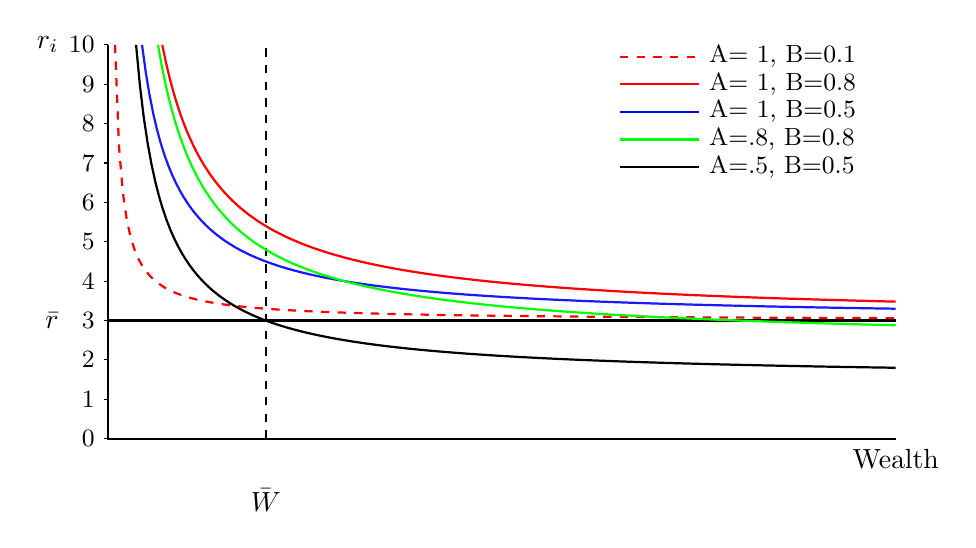
\begin{tikzpicture}[scale=.5]
%\def\bndmax{5}        %https://tex.stackexchange.com/questions/68462/filling-a-complex-region-with-tikz
%\def\bndmin{0.2}
\def \Y {10}  % height of y axis pecent
\def \W {20}  % length  of x axis
\def \Wbar {4} % jmeam wealth
\def \omega {3} % N.B.:  this is r bar

%Equation   \[ r_i = (A + .5 \frac{\bar{W}}{W_i})\omega\]
\def \Wmin{.63}  %This sets the lower limit fo the 
\def \Wmin{(\B*\Wbar)/(\Y/\omega-\A)} %function to keep in in bounds
	
\tikzset{func/.style={thick}}	

\draw [thick] (0,\Y)node[left=.5cm]{$r_i$} -- (0,0)--(\W,0)node[below]{Wealth};  	% Axes
\draw [thick] (0,\omega)node[left=.5cm]{$\bar r$} -- (\W,\omega);  	% Axes
\draw [thick,dashed] ( \Wbar,0)node[below=.5cm]{$\bar{W}$} -- (\Wbar,\Y);  	% Axes

\foreach \yi in {0,...,\Y} \draw (0,\yi)--(-.1,\yi)node[left]{\small$\yi$};

%     ORANGE
% \def \A {1} \def \B {.8}
% \draw[func,domain=\Wmin:\W, orange] plot [samples=200] (\x,{(\A/\x+\B*\X/\Wbar/\x)*\omega});
% \def \A {1} \def \B {.1}
% \draw[func,domain=\Wmin:\W, orange, dashed] plot [samples=200] (\x,{(\A+\B*\X/\Wbar/\x)*\omega});

%     RED
\def \A {1} \def \B {.8}
\draw[func,domain=\Wmin:\W, red] plot [samples=200] (\x,{(\A+\B*\Wbar/\x)*\omega});
\def \A {1} \def \B {.1}
\draw[func,domain=\Wmin:\W, red, dashed] plot [samples=200] (\x,{(\A+\B*\Wbar/\x)*\omega});

%.    BLUE
\def \A {1} \def \B {.5}
\draw[func,domain=\Wmin:\W, blue!90] plot [samples=200] (\x,{(\A+\B*\Wbar/\x)*\omega});
%     GREEN
\def \A {.8} \def \B {.8}
\draw[func,domain=\Wmin:\W, green] plot [samples=200] (\x,{(\A+\B*\Wbar/\x)*\omega});
%.    BLACK
\def \A {.5} \def \B {.5}
\draw[func,domain=\Wmin:\W, black] plot [samples=200] (\x,{(\A+\B*\Wbar/\x)*\omega});


\draw [red,  thick](13, 9)--(15,9)node [right, black] {\small A=\ 1,\ B=0.8};
\draw [red,  thick, dashed](13, 9.7)--(15,9.7)node [right, black] {\small A=\ 1,\ B=0.1};
\draw [blue,  thick](13, 8.3)--(15,8.3)node [right, black] {\small A=\ 1,\ B=0.5};
\draw [green, thick](13, 7.6)--(15,7.6)node [right, black] {\small A=.8, B=0.8};
\draw [black, thick](13, 6.9)--(15,6.9)node [right, black] {\small A=.5, B=0.5};
\end{tikzpicture}


% Figure of cost of borrowing
\caption{Borrowing cost for  $A=1$  $B=0.5$ (blue);  $A=1$  $B=0.8$ (red);  $A=.8$  $B=0.8$ (green);}
\label{Fig:CapitalCost}
\end{center}
\end{figure}
If the expected return on a property is greater than the individual cost of borrowing, it would pay any agent to borrow as much as possible and purchase properties as they can available.\footnote{As pointed out previously,  Equation~\ref{Eqn:DecisionRule} implies a `bang-bang' control - with all sales going to the richest participant unless there are limits on the size of capital flows. For our simulation, we implement such limits. } 
 
The borrowing of most agents will be constrained. A common rule is that mortgage payments cannot exceed some fraction of disposable income. The wealthy will be able borrow larger amounts and at lower interest rates than the less wealthy. 

%The model has been set up so that all of a workers's  income is spent on  basic living costs, $\omega$, transportation $td$ or rent. Disposable income for agent $i$ is therefore just the return  $\omega W_i$ on  financial assets.  


\section{The period and time value of money}
In developing the model we introduced a number of rates, such as $r_i$, the rate that individual $i$ pays for a single borrowing period. The payment calculation is made for a period of length $T$, which we refer to as a mortgage term.
%This means the actual interest paid is a compounded interest rates (VARIABLES LIST FOR THIS).

%In developing the theoretical model we introduced a number of rates, such as $r_i$, the rate that  individual $i$ pays for a single period of borrowing. We assume the calculations are for a  period of length  $T$, which we refer to as a mortgage term. This means that the rates in equations such XXXXX are actually compounded rates.
Taking a simplified example, if the rate is $x$/year, interest payments are $xM$, a share of the total mortgage amount borrowed, $M$, for each of $T$ years. 
If the interest payments are all made at the end of the mortgage term, the lender will require interest on the deferred interest, so agent $i$'s payment at the end of the period $T$ will be:

\begin{align*}
\text{Payment} &= (1+r_i)M                                 \\ 
    &= M + xM(1+x)^{T-1}+ xM(1+x)^{T-2}\dots + xM(1+x)^{0} \\
    &= M\left(1+ x\sum_{z=T-1}^0(1+x)^{z}\right).          \\ 
\end{align*}
Therefore, the interest payment is:
\begin{align*}
r_i.   &=x\sum_{z=T-1}^0(1+x)^{z}.
\end{align*}

For the sake of notational simplicity and clarity of exposition,  we omit the compounding formula throughout our discussion. This means that, while banks may quote a per period interest rates, the equations use a compounded rate. In the computational model we employ the appropriately compounded values. All %the rates are compounded in this way to provide a per-period rates, including all 
 the interest rates, the $r$'s, are compounded in this way, because they require annual or monthly payments at their stated rates.
 It does not affect the discount rates, the $\delta$'s, or the borrowing ratio $m_i$, because they are initially calculated for the term and don't require the same period payments.
 The discount factor $\delta_i$ is always a compounded version of $x$:
 \[\delta_i=\left(\frac{1}{1+x}\right)^T\].
%is a feature of the individual, so it is not affected in this way.
%The appropriate compunding expressions for other rates are displayed below.

 The {mortgage term}, $T$, is the period after which the mortgage must be repaid with interest. We work with a mortgage terms for two reasons. First, in the theoretical analysis, by transforming the multi-period transaction to a single period, we simplify the comprehensibility of the analysis. Second, it reflects the fact that in practice agents  likely consider the profitability of a purchase for a finite term longer than one period. The term period lets them consider the time cost of money in their analysis in a natural way. Parameters for their discounting rates and the term considered can be used to explore the effect of borrowing costs and their personal discounting rates on their decisions. Future interest rates are also not fully known. In the future, we can also vary the compound interest rates to explore the impact of uncertainty, given agents' guesses about the future, and their level of risk aversion.

\section{The owner's decision to sell}
We will assume, at least initially, that for owners, deciding to sell is a life-cycle decision: home owners-workers  reach the end of their working lives, no longer need access to the central city, and put their homes on the market, making room for new workers to enter the urban market.\footnote{The timing decision can be randomized, but that is highly unlikely to affect results. On the other hand, 
\color{red}
if worker-owners remain in their homes after retirement, there are fewer homes available for new workers, which must produce a labour shortage in this model, driving up wages, leading to higher bids and rising home prices, which in turn attracts  speculative bidding. This will only accelerate any shift in the ownership pattern. Our core model suppresses labour market dynamics and the effect of housing shortages to focus on the warranted prices, which are driven by aggregation economies. 
\color{black}} 
\footnote{\color{blue}As a second step, we may allow potential buyers  to approach potential sellers who have not listed with an offer and allow worker-owners to consider retiring early or becoming tenants if an offer is attractive.  This is only likely if speculative pressures are strong. It may require having multiple institutional buyers to make offers more competitive. In that case initial offers will be closer to the maximum bid price, tending to pull prices up and benefit potential sellers.\color{black}}  

Worker-owners in the final few years of their working life may decide to  list if  they notice that the expected price posted by the real estate agent, $P_M^e$,  exceeds (say) 95\% of their reservation price. This is a `hopeful' listing, `fishing' for an offer that exceeds the actual reservation price.

\[P^{ask}>P_M^e> 0.95 P^r\]
Otherwise
\[P^{ask}> 0.10P^r>P_M^e\]
If no offer exceeds the reservation price, no sale is made.

Once an owner reached retirement age, if no sale is made the reservation price is reduced for the next cycle.

If no sale is made the owner considers becoming a landlord. if the present value of net rent is above the reservation price, the owner rents out the home. .

\section{REDUNDANT Financialized capital}
%Individuals and institutions play a role in the housing market through credit markets and direct investment.Agent's access credit shapes worker's ability to purchase homes. Credit is offered by institutions.
% Agents may be able to foresee future growth. %They may even over invest if they follow market trends and bubbles form. 
% They can claim a share of the urban wealth as it grows over time by owning the land. 

If the return on housing investments is competitive with alternative investments, capital from institutions and individuals will flow into housing. Institutional investors can purchase housing.  Individual households can also allocate a larger share to housing to capture the returns.
% If the return on investment in housing is competitive with alternative investments, can purchase housing for it's financial return. They can rent housing and sell the asset with appreciation later. We examine the conditions in which this increased demand can drive up prices in the market. 
% Capturing future growth of the city, depending on their foresight - how much does it take to block individuals from gains-- Regime.
% both institutional investors and individual agents can purchase additional housing for it it's return on investment even though they don't need it as a place to live. 
% Use value vs rent value. 
%Institutional investors can purchase housing as an investment. Individuals with more wealth may invest 
Households may, for example purchase a larger house than they need, purchasing additional units to rent out, or keep a house after retiring rather than downsizing.  % and individuals with sufficient means can purchase larger homes than they need to benefit from appreciation, or purchase additional units to rent to others. 
% Investors can also purchase housing to claim a share of the future productivity of the city. Individuals and groups can put extra money into housing. Institutional housing providers can buy up the housing supply.
% HYPOTHESIS FEEDBACK LOOP -- FINANCIALIZED INVESTMENT --
%The rise in spending on housing as a proportion of income can be driven by both rising prices (cutting into quality of life) and increasing investment to claim a share of the returns.  -- disaggregate and show the geometry -
% Test how linear is this relationship? 

\subsubsection{Size of mortgage available, $m_i$}
\[m_i= \frac{0.25Y_i}{r_i}\]
where $r_i$ is $i$'s cost of capital, $Y_i$ is $i$'s income.

\subsubsection{Cost of capital $r_i$}
The cost of capital is known to differ for rich and poor. Say for example, the cost of borrowing, $r_i$ for agent $i$ if the base lending rate is $\bar{r}$
 \[ r_i = (A + B \frac{\bar{W}}{W_i})\bar r\]
where $\bar{W}$ is mean wealth and $W_i$ is individual wealth. %Figure~\ref{Fig:BorrowingCost} illustrates the effect.

% \begin{figure}[htb]
% \begin{center}
% 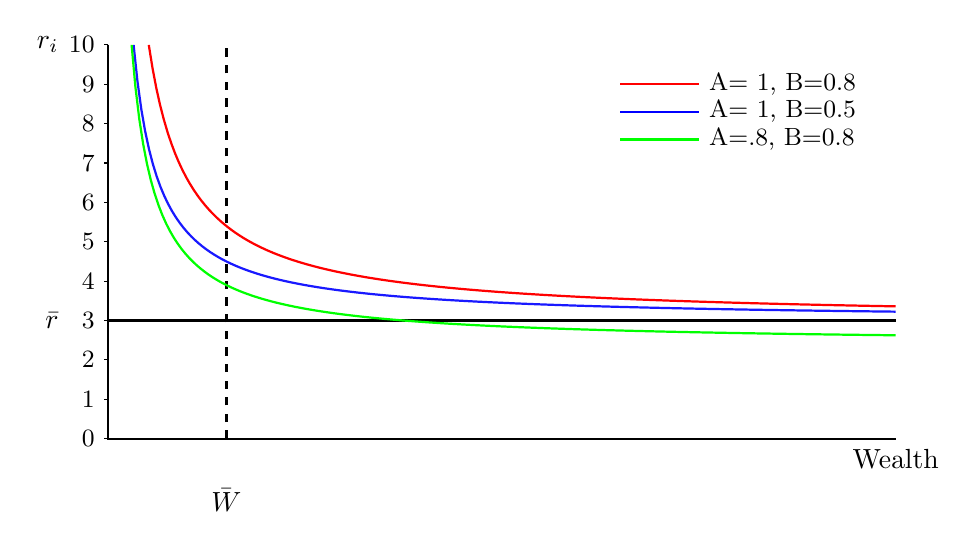
\begin{tikzpicture}[scale=.5]
%\def\bndmax{5}        %https://tex.stackexchange.com/questions/68462/filling-a-complex-region-with-tikz
%\def\bndmin{0.2}
\def \Y {10}  % height of y axis pecent
\def \W {20}  % length  of x axis
\def \Wbar {3} % jmeam wealth
\def \omega {3}
\def \A {1}  %was .5
\def \B {.5}
%Equation   \[ r_i = (A + .5 \frac{\bar{W}}{W_i})\omega\]
\def \Wmin{.63}  %This sets the lower limit fo the 
\def \Wmin{(\B*\Wbar)/(\Y/\omega-\A)} %function to keep in in bounds
	
\tikzset{func/.style={thick,color=blue!90}}	

\draw [thick] (0,\Y)node[left=.5cm]{$r_i$} -- (0,0)--(\W,0)node[below]{Wealth};  	% Axes
\draw [thick] (0,\omega)node[left=.5cm]{$\bar r$} -- (\W,\omega);  	% Axes
\draw [thick,dashed] ( \Wbar,0)node[below=.5cm]{$\bar{W}$} -- (\Wbar,\Y);  	% Axes

\foreach \yi in {0,...,\Y} \draw (0,\yi)--(-.1,\yi)node[left]{\small$\yi$};

\draw[func,domain=\Wmin:\W] plot [samples=200] (\x,{(\A+\B*\Wbar/\x)*\omega});
\def \A {.8}
\draw[func,domain=\Wmin:\W, green] plot [samples=200] (\x,{(\A+\B*\Wbar/\x)*\omega});

\def \A {1}
\def \B {.8}
\draw[func,domain=\Wmin:\W, red] plot [samples=200] (\x,{(\A+\B*\Wbar/\x)*\omega});

\draw [red,  thick](13, 9)--(15,9)node [right, black] {\small A=\ 1,\ B=0.8};
\draw [blue,  thick](13, 8.3)--(15,8.3)node [right, black] {\small A=\ 1,\ B=0.5};
\draw [green, thick](13, 7.6)--(15,7.6)node [right, black] {\small A=.8, B=0.8};
\end{tikzpicture}

% \caption{Hypothetical wealth-dependent borrowing cost}
% \label{Fig:BorrowingCost2}
% \end{center}
% \end{figure}%

This has a number of immediate implications. First, if agents discount at their borrowing rate, wealthier agents a lower discount rate and therefore value properties more highly. 

Second, given the  common rule that mortgage payments cannot exceed some fraction of disposable income, the wealthy will be able borrow larger amounts and at lower interest rates that the less wealthy. At any distance from the centre they will be able to make a higher bid.
 
If the expected return on a property is greater than the individual cost of borrowing, it would pay any agent to borrow as much as possible and purchase properties as they become available.

\subsubsection{The rate of return on a property purchase $v$}
To explore the implication of the financialization of the urban land market we need a function to calculate the return on a unit of land that reflects the actual gradient of opportunity in financial markets. We begin with the price appreciation, $\Delta P=P_T-P_0 = (1+\dot p)P_0-P_0 $, where $\dot p$ is the rate of price appreciation over the period $T$. Rates will all be specified for the period $T$. Transaction costs, including real estate fees, take a fraction from the value of the final sale.

 The speculator invests a down payment, $D$, and gets back at time $T$ the  increased price $(1+\dot p)P_0$, plus rents, minus any costs and minus the mortgage with interest.
%footnote{We can include a use value, $U$ in place of rent for expatriate owners to represent using the property - say one month a year - when they are not renting the property and a \textbf{vacancy tax},
%$T$ at rate $t$ to affect the speculator's  decision.
 
The rate of return is the value of the gain, $V$,  over the size of the downpayment, $D$, where
\begin{equation}https://quoteinvestigator.com/2015/08/30/practice/
V =capital\ gain - Interest\ due  	+ Rent  - operating\ cost\    
\end{equation}

The rate of return is $v = \frac{V}{D}$. 

Both the  share of the price  that can be mortgaged, $m$, and the interest rate  and $r$ may be functions of the agent's wealth. $\delta$ represents the net capital gains tax. It makes it possible to capture the capital gains kept. If it is set to one, it simplifies the equations, all is kept. Keeping the variable offers a policy variable to control the return on financial capital.

\begin{eqnarray*}
V  %	&=& capital\ gain - Interest\ due  	+ Rent  - operating\ cost\\
% 	&=& \delta P_T-D \qquad \qquad \quad - (1+\delta r)M \quad	 + R  	-C\\
% 	&=& \delta P _T \qquad-(P_0-M) \quad- (1+\delta r)M 	 + R  	-C\\
%	&=& \delta (1+\dot p)  P_0 -(P_O -M)  -(1+\delta r)mP_0  + R  -C\\
%	&=& \delta (1+\dot p)  P_0 -P_O + M \qquad -(1+\delta r)mP_0  + R -C\\
%	&=&( \delta (1+\dot p)-1)  P_0  + mP_0 \quad -(1+ \delta r)mP_0  + (\rho-\kappa)P_0\\	
%	&=& \left(  \delta (1+\dot p)-1    + m \quad - m(1+\delta r)  + (\rho-\kappa)\right)P_0\\'
%	&=& \left(  \delta (1+\dot p)-1    + m \quad - m-\delta rm  + (\rho-\kappa)\right)P_0\\
&=& \delta(P_T- (1+r)M) \qquad \qquad 	 + R  	-C   - T\\
&=& \delta((1+\dot p)  P_0- (1+r)mP_0)   + \rho P_0  	-\kappa P_0 - tP_0\\
&=&( \delta((1+\dot p)  - (1+r)m) \ + \rho   	-\kappa -t) P_0
\end{eqnarray*}

This is the  net present value of buying, and selling after one period. \textbf{It has  6 exogenous parameters}. Operating revenue and costs $ \rho -\kappa - t$ a present value. 

The rate of return is $v = \frac{V}{D}$. For expat investors, we get a \textbf{decision rule}:\begin{enumerate}
\item  if $v \geq a$ (with some private use?) with no rent,  don't bother renting. 
\item If $v(no\ rent\ and\ tax) < a\leq v(with\ rent)$,  then  rent. 
\item If $ v(with\ rent) \le a $,  then sell 
\end{enumerate}

We can, with some simplifications, write
\begin{eqnarray}
\frac{V}{D}&=&( \delta((1+\dot p)  - (1+r)m) \ + \rho   	-\kappa - t ) \frac{P_0}{D}   \nonumber\\
		&=&( \delta((1+\dot p)  - (1+r)m) \ + \rho   	-\kappa - t ) \frac{P_0}{P_0-mP_0}   \nonumber\\
		&=&\frac{ \delta(1+\dot p  - (1+r)m) \ + \rho   	-\kappa - t } {1-m} \label{Eqn:DecisionRule}
\end{eqnarray}

\subsubsection{Returns on capital are higher for wealthy investors}
\begin{figure}[htb]
\begin{center}

% Large version
% \begin{tikzpicture}[scale=.5]
% %\def\bndmax{5}        %https://tex.stackexchange.com/questions/68462/filling-a-complex-region-with-tikz
% %\def\bndmin{0.2}
% \def \Y {10}  % height of y axis pecent
% \def \W {20}  % length  of x axis
% \def \Wbar {3} % jmeam wealth
% \def \omega {3}
% \def \A {1}  %was .5
% \def \B {.5}
% %Equation   \[ r_i = (A + .5 \frac{\bar{W}}{W_i})\omega\]
% \def \Wmin{.63}  %This sets the lower limit fo the 
% \def \Wmin{(\B*\Wbar)/(\Y/\omega-\A)} %function to keep in in bounds
	
% \tikzset{func/.style={thick,color=blue!90}}	

% \draw [thick] (0,\Y)node[left=.5cm]{$r_i$} -- (0,0)--(\W,0)node[below]{Wealth};  	% Axes
% \draw [thick] (0,\omega)node[left=.5cm]{$\bar r$} -- (\W,\omega);  	% Axes
% \draw [thick,dashed] ( \Wbar,0)node[below=.5cm]{$\bar{W}$} -- (\Wbar,\Y);  	% Axes

% \foreach \yi in {0,...,\Y} \draw (0,\yi)--(-.1,\yi)node[left]{\small$\yi$};

% \draw[func,domain=\Wmin:\W] plot [samples=200] (\x,{(\A+\B*\Wbar/\x)*\omega});
% \def \A {.8}
% \draw[func,domain=\Wmin:\W, green] plot [samples=200] (\x,{(\A+\B*\Wbar/\x)*\omega});

% \def \A {1}
% \def \B {.8}
% \draw[func,domain=\Wmin:\W, red] plot [samples=200] (\x,{(\A+\B*\Wbar/\x)*\omega});

% \draw [red,  thick](13, 9)--(15,9)node [right, black] {\small A=\ 1,\ B=0.8};
% \draw [blue,  thick](13, 8.3)--(15,8.3)node [right, black] {\small A=\ 1,\ B=0.5};
% \draw [green, thick](13, 7.6)--(15,7.6)node [right, black] {\small A=.8, B=0.8};
% \end{tikzpicture}


\[   r^h=\frac{ \delta(1+\dot p  - (1+r)m) \ + \rho   	-\kappa - t } {1-m}    \]
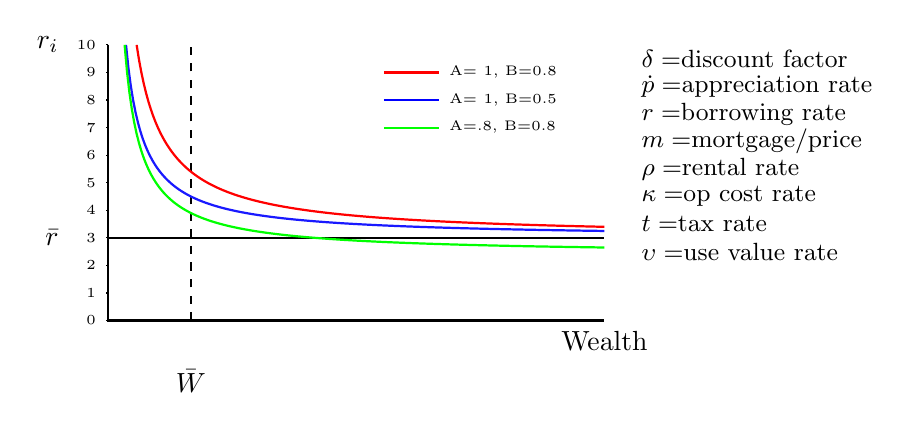
\begin{tikzpicture}[scale=.35]
%\def\bndmax{5}        %https://tex.stackexchange.com/questions/68462/filling-a-complex-region-with-tikz
%\def\bndmin{0.2}
\def \Y {10}  % height of y axis percent
\def \W {18}  % length  of x axis
\def \Wbar {3} % j mean wealth
\def \omega {3}
\def \A {1}  %was .5
\def \B {.5}
%Equation   \[ r_i = (A + .5 \frac{\bar{W}}{W_i})\omega\]
\def \Wmin{.63}  %This sets the lower limit fo the 
\def \Wmin{(\B*\Wbar)/(\Y/\omega-\A)} %function to keep in in bounds
	
\tikzset{func/.style={thick,color=blue!90}}	

\draw [thick] (0,\Y)node[left=.5cm]{$r_i$} -- (0,0)--(\W,0)node[below]{Wealth};  	% Axes
\draw [thick] (0,\omega)node[left=.5cm]{$\bar r$} -- (\W,\omega);  	% Axes
\draw [thick,dashed] ( \Wbar,0)node[below=.5cm]{$\bar{W}$} -- (\Wbar,\Y);  	% Axes

\foreach \yi in {0,...,\Y} \draw (0,\yi)--(-.1,\yi)node[left]{\tiny$\yi$};

\draw[func,domain=\Wmin:\W] plot [samples=200] (\x,{(\A+\B*\Wbar/\x)*\omega});
\def \A {.8}
\draw[func,domain=\Wmin:\W, green] plot [samples=200] (\x,{(\A+\B*\Wbar/\x)*\omega});

\def \A {1}
\def \B {.8}
\draw[func,domain=\Wmin:\W, red] plot [samples=200] (\x,{(\A+\B*\Wbar/\x)*\omega});

\draw [red,  thick](10, 9)--(12,9)node [right, black] {\tiny A=\ 1,\ B=0.8};
\draw [blue,  thick](10, 8)--(12,8)node [right, black] {\tiny A=\ 1,\ B=0.5};
\draw [green, thick](10, 7)--(12,7)node [right, black] {\tiny A=.8, B=0.8};

\def \W {19}  % length  of x axis
\node[right] at (\W,9.5){\small$\delta=$discount factor};
\node[right] at (\W,8.5){\small$\dot p=$appreciation rate};
\node[right] at (\W,7.5){\small$r=$borrowing rate};
\node[right] at (\W,6.5){\small$m=$mortgage/price};
\node[right] at (\W,5.5){\small$\rho=$rental  rate};
\node[right] at (\W,4.5){\small$\kappa=$op cost rate};
\node[right] at (\W,3.5){\small$t=$tax rate};
\node[right] at (\W,2.5){\small$\upsilon=$use value rate};
 \end{tikzpicture}


\caption{Hypothetical wealth-dependent borrowing cost}
\label{Fig:BorrowingCost}
\end{center}
\end{figure}%



\chapter{Implementation: Relating the market model to the code}
The chapter links the theory to the output of the simulations. %is intended to explain the code and justify the modeling decisions that link the theory to the actual 


\section{MOVE UP? Bargaining - The market process and bargaining}
We consider a homogeneous city with a single wage, identical preferences, uniform identical transportation costs, identical lot sizes.

Individuals and institutions buy and sell properties given individual goals, resources and available information.

% The process can be summarized as
The model of the market process includes the following steps:
The core machinery of the model is the market process. At the centre of that process is a model of price formation and bargaining. % bargaining model. 

\begin{enumerate}
    \item Identify the set of sellers for the current cycle. This may include:
    \begin{enumerate}
        \item people retiring in this cycle,
        \item people who retired and failed to sell, and potentially
        \item people approaching retirement who might consider selling early and
        \item financialized owners. % the bank? speculative owners? .
    \end{enumerate}
    
    \item For each seller, calculate the expected property price: % \textbf{from real estate agent}:
    \begin{enumerate}
        \item Initialize with the warranted price, which is the value of the stream of services, provided by the property. Rents minus net costs:
       \[ P_W=\frac{(\omega-{dc}) + {a}\psi}{r}\]
        The value of the house is the rent premium minus the cost of transportation. Subtract the costs of running the house, divided by the interest rate
    
        IS IT MINUS A $\psi$ SINCE HIGHER COSTS LOWER PRICES?
       
        {\color{green} This is the expected warranted price. It might make sense just to use the homeowner's reservation price (maximum bid price)}.
        \item in later cycles use the actual transaction price $P_M$ (with inflation added) when it is available, or use a (regression)estimate $P_{it}^e$ the real estate agent.
    \end{enumerate}
    
    \item for each seller, compute a reservation price using a variant of the maximum bid price formula. 
    {\color{green}\textit{Values like $m_i$ are going to be expected values for others.  ??? }}
    \textit{This is what the seller thinks she should get, taking into account her expectations about the price increase etc..}
    
    \item for each seller, compute an asking price. 
    \textit{Add some percentage to the reservation price. Make sure the result is above ***? $P_M^e$, since you know you might have to come down in bargaining.}   
    
    \item for each seller, list the asking price for bidders to see.
    
    \item for each property, identify a set of potential bidders.
    \begin{enumerate}
        \item Bank considers bidding on all listed properties.
        the formula is the maximum bid price with its own parameters putting in the current rents.
        \item New entrants to labour market
       {\color{yellow} \item Retirees who might sell, move out of town and invest in a rental property}
    \end{enumerate}
    
    \item for each bidder, compute a maximum price using a variant of the bid price formula. 
    
    \item for each bidder, compute an initial bid no higher than  the maximum price. 
    \color{red}  
    \textbf{(there may be two paths to consider: working from initial bids, or working with max bids )}
    
    \item With list of max bids, check to see if any exceed the asking price. 
    \begin{enumerate}
        \item If yes settle on asking price if there is just one, and the second highest max bid if there are more than one.
        \item If no, proceed.
    \end{enumerate}
    
    \item With list of max bids, check to see if any exceed the reservation price. 
    \begin{enumerate}
        \item If no, house is not sold, and reservation price is reduced for the next cycle.
        \item if one max exceeds the reservation price,  split the difference between the reservation price and the maximum bid bid.
        \item if more than one max exceeds the reservation price, choose the second highest max bid if there are more than one
    \end{enumerate} 
\end{enumerate} \color{black}


-----

All agents have access to the price forecast, $P_M^e$, from the real estate agent.

We have five categories of potential buyers.\footnote{Types three and four  would  become landlords if the transaction is completed, which is a change of class status.} 
\begin{enumerate}
    \item newcomers to the city, who have a job offer  and seek to buy a home or become tenants.  
    \item financial investors who possess financial capital and seek a rate of return better than they would receive from alternative investments. We refer to this investor as `the bank'
    \item owner-occupiers who might mortgage their current homes  to purchase a revenue property
    \item owner-workers who retire and might  invest in a revenue property rather than spending  their capital gain 
    \item sellers are also default buyers, since they can buy their own home and rent it out if their \gls{reservation price} is not met.  
\end{enumerate}


For potential sellers the maximum bid price is also the `\gls{reservation price}' price.  
\[P^{ask}> P^r, \qquad   P^{offer}< P^{max}\]


All potential buyers and potential sellers  will calculate a \gls{maximum bid price} or reservation price and and an initial offer price or ask price \gls{bid  price}. 

The initial bid price (offer) will be lower than the potential buyers maximum bid price. The initial ask price will be higher than the reservation price.

Bargaining will occur when the maximum bid price of at least one agent exceeds the reservation price of the listing agent.

Transactions can occur when the maximum bid price of at least one agent exceeds the reservation price of the listing agent.


\subsection{Determining initial offer and ask prices}

Agents can calculate their maximum bid  or their  reservation price. 
These values are not public. We need to identify initial ask and offer prices, which is the way they appear in the market.


\[P^{ask}> P^r> P_M^e\] 

If the posted expected price exceeds their \gls{reservation price} they 
\begin{enumerate}
    \item list  the property for sale.with the real estate age,nt.
    \item select and asking price   
\end{enumerate}

The bank posts a \gls{maximum bid function} with the real estate agent.

In practice, potential investors will make an  initial  bid that is lower than this value and subsequent bargaining will settle of a price between the initial bid and the seller's asking price.

In the market, the initial bid should be smaller than the bid price calculated, which is a maximum that can earn the target rate of return, The bank will definitely go this high. 

If there is a  max bid among competing buyers, the second highest max bid should be the sale price, but the bidder with the highest max bid wins the property. This is realistic because in a bidding war the final bid only has to be a very small amount higher than that of the last competitor left.
That is the highest price that a seller can get.

 %This  seems realistic enough and is very simple to implement. It should producer a path that is indistinguishable form any more complex approach. 

% Will persons retiring who would leave the city invest in an urban rental?



% But what is $D$? Does the bank have unlimited funds? Isn't D just a fraction of P?  If so it cancels out
% r is the prime rate- that the bank pays? 



% \begin{verbatim}
% \end{verbatim}

\section{Computing values for bid and warranted price}

In the following sections we discuss % the computation of agents' bid price, outline potential discounting approaches, and discussing 
how each component of the calculation is treated in the code. %, organizing the discussion following Equation~\ref{eqn-bid-price2}:


\begin{align}
P_i^{bid} \le   \frac{\mathcal{R}_N}{(1-m_i)r_i^{target}- \delta_i \left(1+L(P)- (1+ r_i)m_i\right)}.
\end{align}
Net rent, $\mathcal{R}_N$, is discussed in section \ref{SS:NetRent}. 

Interest rates, discount rates, and borrowing ratios are discussed in section \ref{SS:RatesAndRatios},
The borrowing ratio, $m_i$, is discussed in section \ref{SS:BorrowingRatio}, the target interest rate, $r_i^{target}$, is discussed in \ref{SS:targetr} the discount factor, $\delta_i$ is discussed in section \ref{SS:discountfactor}. The price approximation mechanism, $L(P)$ is discussed in \ref{SS:PriceForecast}, and the interest rate the buyer has to pay for the mortgage, $r_i$, is discussed in \ref{SS:BankRate}. Sections are thus numbered: 

\begin{align*}
P_i^{bid} \ge   \frac{\ref{SS:NetRent}} {(1-\ref{SS:BorrowingRatio})\ref{SS:targetr}-
\left[ \ref{SS:discountfactor}(1+\ref{SS:PriceForecast}- (1+\ref{SS:BankRate})\ref{SS:YWealthConstraint})\right]}. 
\end{align*}


\section{CODE DISCUSSION}
present value of tax on propriety over T years. 

\section{Operating cost calculations}
\begin{verbatim}
property value * tau * (sum_(1-T) ((1/(1+r))^t).    
    (sum_(1-T) ((delta_t)

psi   = 100000 # subsistence wage
    
#  Annual operating cost in dollars  
#  eg psi=100000 b=.02 , a*b*psi= 2000 per year 

 compounded for 5 years Must add the discount factors  
 \delta_t for five years 
 \[ oppcost=  \[\frac{\omega+a\phi}{r} \tau + a\phi b\right]\sum_1^T \frac{1}{1+r}\]
 a*b*psi/.r - (a*b*psi/r)*delta_T
#  eg   2000/.r - (2000/r)*delta_T 
= 2000/0.05 - (2000/0/05)*delta_T = 8658.953

opperating_cost = a*b*psi/r - (a*b*psi/r)*delta_T 
\end{verbatim}

\[ oppcost=  \left(\tau\omega  +(\tau+b)a\psi\right)\sum_1^T \left(\frac{1}{1+r}\right)^t\]

\begin{verbatim}
    opperating_cost = (tau*(omega-c*d) + (tau+b) *a*psi)* sum((1/r)^t for t in range(1, T))
    
This is (tax on rent plus both tax and maintenance on the house and land) for (T years with discounting for each year),
\end{verbatim}



----


The relationship between income and consumption is suppressed, because that makes xyz.. so much clearer.

because it ignores
but the relationship

but the relation ship between x and y is not..

don't care what they do in retirement, so ignoring it, so they're still capturing capital gains so long as they own a house
t
their lifetime income is changing even though their current income is not.

--
renters get none of that.



$delta_T$ 
$sum_delta_T$
% $sum_r_T$

$r_T$  present value of total interest payments made over period T




${a}$  =  share of subsistence wage  used for land and building e.g. 0.3

${b}$  = share of share of subsistence wage  used on maintenance e.g. 0.2

${c}$  = annual tax rate on rent and home  e.g. 12 mills 


a     share of subsistence wage  used for land and building

b      share of share of subsistence wage used for maintaining home

c    annual tax rate on rent and home  eg  1.6\% = 16 mills, 1.2\% =.12 mills

% Sigma is tax share, what is the tax rate.
% delta is density ** - - infinitesmal density increase as the city moves out. [[adjustment speed for wage N]] imagine a density function over the city. 

\section{SORT Housing services 30 percent}
MOVE TO ASSUMPTIONS - We assume households spend a fixed fraction $a$ of their subsistence wage $\psi$ on housing. 

\footnote{***JUSTIFY ASSUMPTION OF FIXED SHARE OF SUBSISTENCE HERE? This appears to be empirically justified and simplifies the model \cite{SOURCE_HOUSING_A_FIXED_SHARE_SUBSISTENCE_WAGE}. Appendix \ref{appendix-future-work} considers how the assumption may be relaxed in future work.}

Housing services absorb about 30\% of income  we will use than number  as an approximation,  $a\psi$, where $a$ is the share of the subsistence wage and $\psi$

Note, this is a simplification. It ignores any locational values of the house, as well as the costs stream, it is a net cost, but a net cost embedded in the share of the income. It is a justified simplification, but an interesting place to explore the effect of adding nuance.  MAYBE MOVE DISCUSSION OF POTENTIAL EXTENSIONS TO FUTURE WORK.

\section{Net rent}\label{SS:NetRent}
We assume that the present value of the rent % $\mathcal{R}$ 
is known to an investor in advance. We can imagine the investors' accountant having information on the rent that the market will bear or on prior rents and including this information in the calculation of $P_B$.

Uncertainty can be represented as bias or stochasticity.
Calculation notes: I have rent from the wages. I have kappa and sigma from our ex parameter values. . omega from the wages. 

Net rent, which can be written a share, $\phi$ of total rent $\mathcal{R}_N = \phi \mathcal{R}$
$\mathcal{R}_N = \phi \mathcal{R}$

Where the \gls{rent share}, phi is a fraction
$\phi = (rent-taxes-costs) /rent$ 

There's a distinction between the warranted rent, the net rent, and the rent that's actually charged.

We assume that the  rent  actually charged to a tenant is the warranted economic rent, ($\mathcal{R}= \omega - {dc}$), but the relevant term to enter into the calculation of return on investment is the net rent $\mathcal{R}_N$ for a given property, because the returns are the returns an investor can get after paying taxes and operating costs.

In our computational model, we do the calculation in terms of a mortgage, so we want the total returns after expenses, in present value, compounded over the mortgage  period.
% We want the total returns after expenses, in present value, compounded over a 5 year period.

\begin{align}
\mathcal{R}_N &= \mathcal{R} - \mathcal{O} - \mathcal{T} 
\end{align}

In terms of the warranted rent, 
\begin{align}
\mathcal{R}_N &= (1-\kappa_j - \sigma_j)(\omega - {dc}) % was {d_j} here
\end{align}


% $\mathcal{R}_N = (1-\kappa_j - \sigma_j) (\omega - {c} d_j)$

% {\color{red}
% Notice that  we need here is really the fraction of the warranted rent that the owner gets to keep after maintenance costs and taxes. It is possible that the owner is charging more or less than the economic  rent, but economic rent can be seen as an equilibrium value. Economic rent is $\mathcal{R}$.  This is (tautologically) related to the price as a fraction of the actual sale price: COULD MOVE TO THE CHAPTER NOW SINCE THE THE SECTION IS MOVED THER
% }
% \[\mathcal{R}= \frac{\mathcal{R}}{P_0}P_0 \]

If we want to know the  present value  of the \textbf{net rent}, $\mathcal{R}_N$  collect over the period  $T$, $\mathcal{R}_N^T$, we \textbf{add up} the discounted rents for each year. We may assume the rents are rising at and that the first is the current warranted rent, which gives us a computational formula. 
\[\mathcal{R}_N^T= (\omega-dc)\sum_{t=0}^{t=T-1} \frac{(1+\dot{\mathcal{R}})^{t}} {(1+r_{r_\delta})^{t+1}} \]

% \[\mathcal{R}_Nj^T= (\omega-dc_j)\sum_{\tau=0}^{\tau=T-1}\left[\frac{1+\dot{\mathcal{R}}}{1+r_{r_\delta}}\right]^\tau \]
\noindent where $\dot{\mathcal{R}}$ is an expected rate of change of rents - possibly zero for now, and $r_\delta$ is the individual's discount rate. 

TODO: problem - how to handle subscripts with net rent $\mathcal{R}_N$


\subsection{Tax ratio}\label{SS:TaxRatio} 
The tax ratio $\sigma$ is the share of rents that the municipality takes for services and infrastructure. This fraction of the value of the property is about 30\% based on mill rates in Ontario,  so $\sigma = 0.3$. % REFERENCE

*** CHECK Total taxes paid on  property $j$, over a given mortgage period $T$ is 

\[\Psi_j^T = \psi * \mathcal{R}\].  

    %\href{https://www.google.com/url?sa=t&rct=j&q=&esrc=s&source=web&cd=&ved=2ahUKEwiOmNPUvIL9AhUUmokEHX-5C9oQFnoECBIQAQ&url=https%3A%2F%2Fwww.greatersudbury.ca%2Fcity-hall%2Ftax-services%2Fpdf-documents%2F2022-tax-rates%2F&usg=AOvVaw2XEdfcC5z-5AqfOeH5t-eN}{Sudbury values}  same as https://www.greatersudbury.ca/city-hall/tax-services/pdf-documents/2022-tax-rates/

\subsection{Cost tax ratio}\label{SS:CostRatio} 
The value of $\kappa$  varies for every property based on maintenance requirements, historic rents, tenant rights, and variations in assessed values. If it varies, it may be useful as a quality indicator.

%Values for $\kappa$ and $\sigma$ must be adjusted to take into account the length of the period or net rents have to be summed over the period.  NO LONGER NEEDED 

Nothing prevents $\sigma+\kappa >1$, which would leave an investor unable to cover building maintenance and taxes out of current rent. 


\section{Income and wealth effects}
\subsection{Interest rates, discount rates and borrowing ratios} \label{SS:RatesAndRatios}

According to the Canada Housing Statistics Program (CHSP), first time home buyers require a combination of sufficient income and savings in order to enter the housing market. (insert tables? from the CHSP?) We have implemented these facts by making interest rates and mortgage share depend on income and wealth.
% image.png

% image.png
% https://www150.statcan.gc.ca/n1/pub/46-28-0001/2023001/article/00001-eng.htm

% Investors now make up more than 25\% of Ontario homebuyers, pushing prices higher, experts warn. 2020

% Released: 2022-04-12

% New data from the Canadian Housing Statistics Program (CHSP) show the extent of inequalities in housing: multiple-property owners possess nearly one-third of all residential properties and the top 10\% wealthiest owners account for around one-quarter of residential housing value. Despite these inequalities, new data show an increase in the number of first-time home buyers from 2018 to 2019.
% Both income and housing wealth are concentrated at the top, even among owners. When ordering individual owners by their yearly incomes, the top 10% of owners in Ontario and British Columbia each had yearly incomes above $125,000.
 

\subsection{Borrowing ratio} \label{SS:BorrowingRatio}
$m_i$

The borrowing ratio, $m_i$, is just the fraction of the price that the bank will lend to a potential buyer. \textbf{It may depend on the individual.} 

Income(\ref{SS:YWealthConstraint}) and/or wealth (\ref {SS:MWealthConstraint}) may constrain individual participation in markets. 
Here we should use the same logic as we use about the interest rate charged. (\ref{SS:BorowingRate})

It is likely to be higher for institutional buyers  and for the wealthy because the bank thinks those with assets are more secure risks. they may have other assets that could be attached in the case of default.
(note interventions with reduces interest rates, or loan assessments drawing on techniques used by foundations could have value)


\subsection{Target interest rate}\label{SS:targetr}

 The target interest rate, $r^{target}$, is the prime rate plus a margin. % required by the bank.  Question: do non-bank actors have such a term?

\begin{verbatim}
self.get-target-interest-rate(buyer)
\end{verbatim}



\subsection{Discount factor}\label{SS:discountfactor}

The discount factor $\delta_i$ for THE END OF period $T$ captures the cost of waiting $T$ periods to sell the property. The usual way to treat it, which we use here, is to assume that $i$ has an interest rate $r_i$ and has been investing efficiently. This means that  the individual has a discount factor for future returns based on the year-over-year rate of return. 

\[\delta^T_i=\left[\frac{1}{1+r_i}\right]^T\]



\subsection{Price forecast approximation} \label{SS:PriceForecast}
$L(p)$

$p$ is all the price data plus any exogenous information (e.g. policy knowledge?). $L(p)$ is an estimation function that produces a `common knowledge' value for the rate of price increase. Later you can add idiosyncratic extra knowledge or extra ignorance.

Some spatial regression references:
'taxonomy of spatial econometric model specifications that incorporate spatial externalities in various ways'
\cite{anselinSpatialExternalitiesSpatial2003},  
overviews of econometric methods and computational tools \cite{anselinModernSpatialEconometrics2014}, \cite{gelmanDataAnalysisUsing2006}.

\subsection{Prime interest rate}\label{SS:BankRate}
$r$

The bank's interest rate, $r$, is just the bank rate (prime rate? set by the Bank of Canada. Exogenous. Just assign  a value like 4\%.

\subsection{Wealth constraint on m} \label{SS:MWealthConstraint}

We can define individual wealth as:
\[W_i= P_i -M_i  +S_i\]
where 

\begin{tabular}{ll}
$P_i$ & value of owned home\\
$M_i$ & Mortgage on owned home\\
$S_i$ & personal savings = $age*d*W$\\
\end{tabular}

The availability of capital differs for rich and poor. 


We can develop an expression to capture the relationship between the \gls{borrowing ratio}, $m_i$,  and individual wealth. Figure~\ref{Fig:Borrowingratio} illustrates a mortgage availability  model that is written:

 \[ m_i = \frac{0.1 \left(9-\left(\frac{W_i}{\bar W}\right)^{0.5}l\right)}{2} \]

 
Where $\bar{W}$ is mean wealth and $W_i$ is individual wealth. 
The relationship is clearly established empirically \cite{}, but location and shape of the curve may vary somewhat. The curve is parameterized, here, so that the bank has a borrowing ratio close to one, perhaps 0.9, since it has many assets. The borrowing ratio for the median wealth holder, perhaps 0.8.


% TODO *** why two axis labels? - and need to label y axis properly

\begin{figure}[htb]
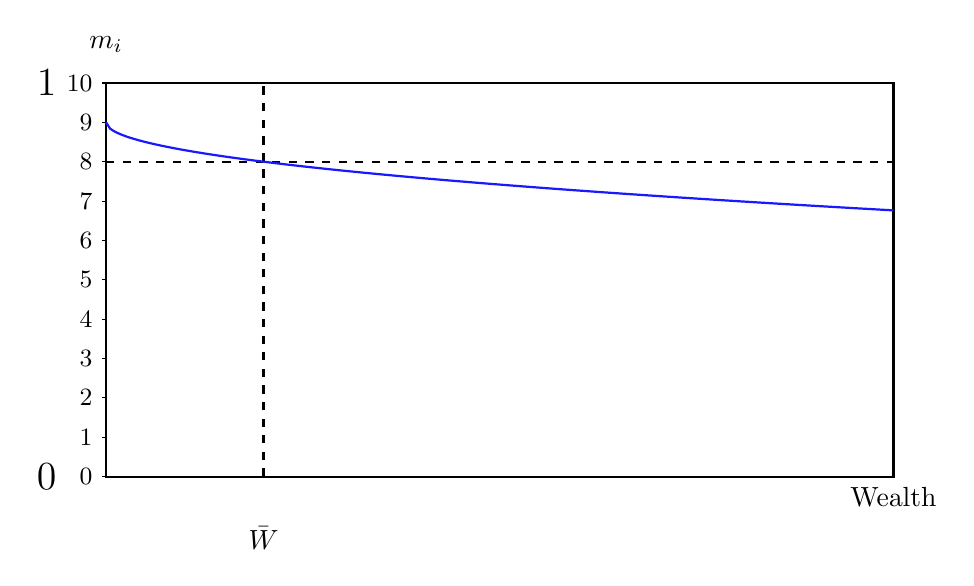
\begin{tikzpicture}[scale=.5]
%\def\bndmax{5}        %https://tex.stackexchange.com/questions/68462/filling-a-complex-region-with-tikz
%\def\bndmin{0.2}
\def\Y{10}  % height of y axis pecent
\def\W{20}  % length  of x axis
\def\Wbar{4}
\def\rbar{8}% this is the prime rate

% %Equation   \[ r_i = (A + .5 \frac{\bar{W}}{W_i})\omega\]
   % \def\Wmin{.63}  %This sets the lower limit fo the 
    \def\Wmin{(\B*\Wbar)/(\Y/\rbar-\A)} %function to keep in in bounds
	
 \tikzset{func/.style={thick,color=blue!90}}	

 \draw [thick](\W,\Y)-- (0,\Y)node[left=.5cm]{\Large$1$}node[above=.25cm]{$m_i$} -- (0,0)node[left=.5cm]{\Large$0$}--(\W,0)node[below]{Wealth}--cycle;  	% Axes box
 
 \draw [dashed, thick] (0,\rbar) -- (\W,\rbar);  	% Axes
\draw [thick,dashed] ( \Wbar,0)node[below=.5cm]{$\bar{W}$} -- (\Wbar,\Y);  	% Axes

\foreach \yi in {0,...,\Y} \draw (0,\yi)--(-.1,\yi)node[left]{\small$\yi$};
%\foreach \yi in {0,2,4,6,8,10} \draw (0,\yi)--(-.1,\yi));
%node[left]{\small$\yi$};
%\foreach \yi in {0,2,4,6,8,10}node at (-.1,yi) {{10*yi}} ;
\draw[func,domain=0:\W] plot [samples=200] (\x,(9-\x^.5/2);

 \end{tikzpicture}
\caption{Individual borrowing ratio $m_i$ as a function of wealth (in tenths)}
 \label{Fig:Borrowingratio}
\end{figure}


\subsubsection{Individualized borrowing rates}\label{SS:BorowingRate}
 
 
 $r_i$ depends on relative income and assets, as well as base interest rates. % compared to others. 
 The median after-tax income of Canadian families and unattached individuals was \$66,800 in 2020 according to Statistics Canada's %\href{https://www150.statcan.gc.ca/n1/daily-quotidien/220323/dq220323a-eng.htm}{Canadian Income Survey, 2020}.  \href{https://www150.statcan.gc.ca/t1/tbl1/en/tv.action?pid=1110005501}
 Data released in 2020 by Statistics Canada indicates that the top 1\% of Canadians made, on average, around \$512,000 in a single year \cite{stats-can-canadian-incomes}. % \href{https://www150.statcan.gc.ca/n1/daily-quotidien/201222/dq201222b-eng.htm}{Survey of Financial Security, 2019}.

 A study by Statistics Canada found that the typical Canadian household now has a median net worth of \$329,900, while the average net worth in Canada is \$738,200 \cite{stats-can-median-net-worth}.  %\href{https://www150.statcan.gc.ca/t1/tbl1/en/tv.action?pid=1110005501}{High income tax filers in Canada}

\subsubsection{Computing the income constraint on interest rates}\label{SS:YWealthConstraint}
$r_i$

In our model, we  tie the individual cost of capital,  $r_i$ for agent $i$, to a prime rate, $\bar r$ or the bank's target rate, $r^{target}$, prime plus 1\%, say. and to individual wealth. Figures~\ref{Fig:Borrowingrate1} and ref{Fig:Borrowingrate1} illustrate a couple of possible  cost-of-borrowing models roughly consistent  with the stylized facts about lenders. 

\begin{align}
 r_i =  &  \left(A + B \frac{\bar{W}}{W_i}\right) \bar r       \label{eq:incomeandr1}  \\
 r_i =  &  \left(\bar r - A + B *\frac{\bar W}{W_i - C}\right) \label{eq:incomeandr2}  \\
\end{align}
Where $\Bar{W}$ is mean wealth and $W_i$ is individual wealth. In Equation~\ref{eq:incomeandr2},  A determines y-shift, B, the scale, and C the  x-shift for the curve.


\begin{figure}
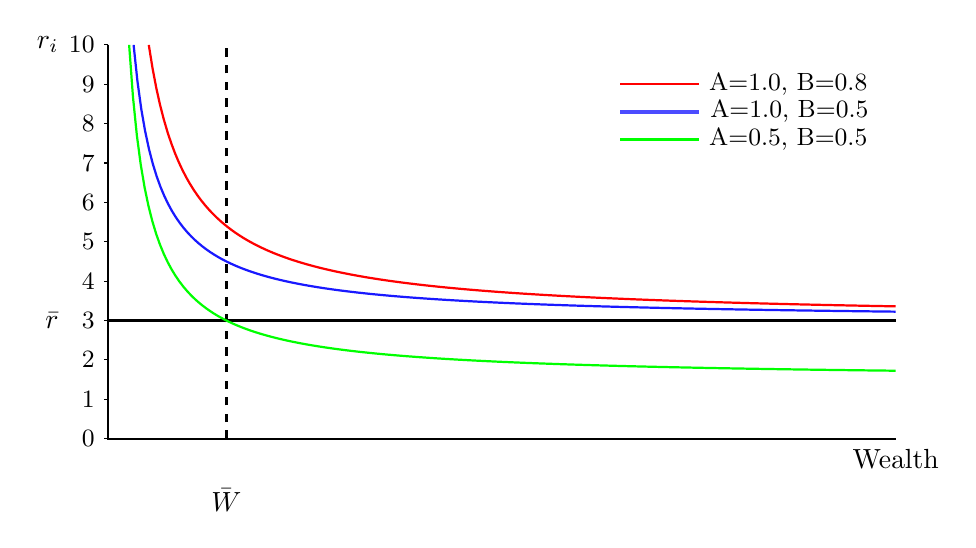
\begin{tikzpicture}[scale=.5]
%\def\bndmax{5} % https://tex.stackexchange.com/questions/68462/filling-a-complex-region-with-tikz
%\def\bndmin{0.2}
\def \Y {10}    % height of y axis as a pecent
\def \W {20}    % length  of x axis
\def \Wbar {3}  % mean wealth
\def \rbar {3}  % the prime rate 

% Equation   \[ r_i = (A + .5 \frac{\bar{W}}{W_i})\omega\]
\def \Wmin{.63}  %This sets the lower limit fo the 
\def \Wmin{(\B*\Wbar)/(\Y/\rbar-\A)} %function to keep in in bounds
\tikzset{func/.style={thick}}	

% Axes
\draw [thick] (0,\Y)node[left=.5cm]{$r_i$} -- (0,0)--(\W,0)node[below]{Wealth};  
\foreach \yi in {0,...,\Y} \draw (0,\yi)--(-.1,\yi)node[left]{\small$\yi$};
\draw [thick] (0,\rbar)node[left=.5cm]{$\bar r$} -- (\W,\rbar);  	% Axes
\draw [thick,dashed] ( \Wbar,0)node[below=.5cm]{$\bar{W}$} -- (\Wbar,\Y);  	% 

\def \A {1.0}  \def \B {0.5} %BLUE
\draw[func,domain=\Wmin:\W, color=blue!90] plot [samples=200] (\x,{(\A+\B*\Wbar/\x)*\rbar});
\draw [ultra thick, color=blue!70 ](13, 8.3)--(15,8.3)node [right, black] {\small A=\A,\ B=\B};

\def \A {0.5} 
\def \B {0.5} % GREEN
\draw[func,domain=\Wmin:\W, color=green] plot [samples=200] (\x,{(\A+\B*\Wbar/\x)*\rbar});
\draw [thick,  color=green](13, 7.6)--(15,7.6)node [right, black] {\small A=\A, B=\B};

\def \A {1.0}  \def \B {0.8} % RED
\draw[func,domain=\Wmin:\W, red] plot [samples=200] (\x,{(\A+\B*\Wbar/\x)*\rbar});
\draw [thick,  color=red](13, 9)--(15,9)node [right, black] {\small A=\A,\ B=\B};
% KEY
\end{tikzpicture}
\caption{Individual borrowing cost as a function of wealth}
\label{Fig:Borrowingrate1}
\end{figure}


\begin{figure}
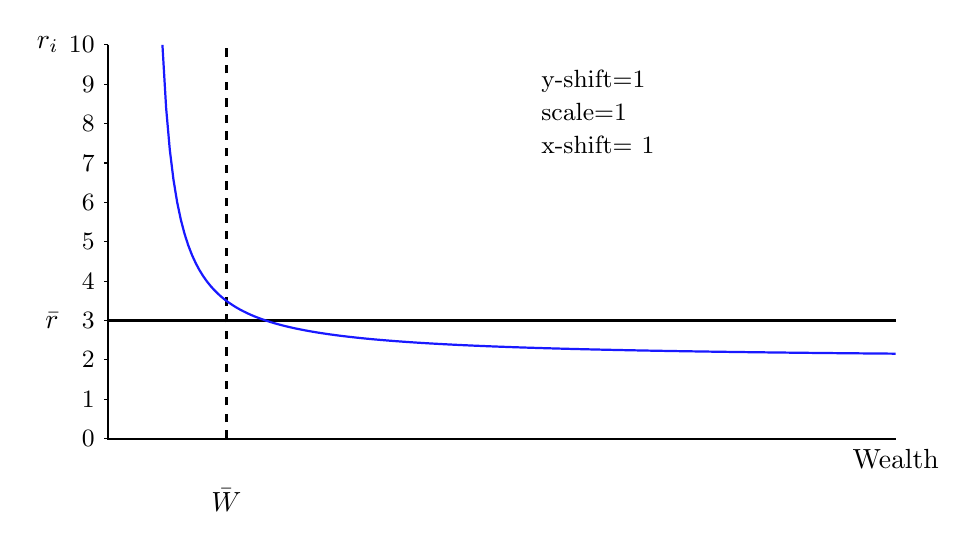
\begin{tikzpicture}[scale=.5]
%\def\bndmax{5}        %https://tex.stackexchange.com/questions/68462/filling-a-complex-region-with-tikz
%\def\bndmin{0.2}
\def \Y {10}  % height of y axis pecent
\def \W {20}  % length  of x axis
\def \Wbar {3} % meam wealth
\def \rbar {3}% this is the prime rate 

%\def \Wmin{(\B*\Wbar)/(\Y/\rbar-\A)} %function to keep in in bounds
\tikzset{func/.style={thick}}	
	% Axes
\draw [thick] (0,\Y)node[left=.5cm]{$r_i$} -- (0,0)--(\W,0)node[below]{Wealth};  
\foreach \yi in {0,...,\Y} \draw (0,\yi)--(-.1,\yi)node[left]{\small$\yi$};
\draw [thick] (0,\rbar)node[left=.5cm]{$\bar r$} -- (\W,\rbar);  	% Axes
\draw [thick,dashed] ( \Wbar,0)node[below=.5cm]{$\bar{W}$} -- (\Wbar,\Y);  	% 

\def \A {1} %vertical shift aroung \rbar, the prime rate
 \def \B {1}  % Scales the exponential curveBLUE
 \def \C {1}  %right shift  
% \def \Wmin {.4+\B}  %This sets the lower limit fo the 
\def \Wmin {(\B*\Wbar)/(\Y-\rbar+\A) +\C} %function to keep in in bounds

\draw[func,domain=\Wmin:\W, color=blue!90] plot [samples=200] (\x,{\rbar-\A+\B*\Wbar/(\x-\C))});
\node  [align=left, text width =2cm ] at (13, 8.3) {\small y-shift=\A \newline scale=\B \newline x-shift= \C};

 \end{tikzpicture}
\caption{Individual borrowing cost as a function of wealth II}
\label{Fig:Borrowingrate2}
\end{figure}

The rates $\delta,\ \sigma,$ and $r$ depend on the period, $T$. 

\subsection{Incorporating growth and discounting}
%We need a time period T for calculations. For use in any calculation, 

With a price-growth rate of $\dot P$ per year, the growth over $T$ years is $(1+\dot P)^T$, and  %and a 5 year mortgage period, 
the expected price at the end of the period is:

\[P_M^{Te}=P_0(1+\dot P)^T\]

If, for example price growth is 10\%, $\dot P= 0.1$, the {capital gain}, or growth, over a 5-year mortgage term is 0.61051 $\approx$ 60\% of the original price, $P_0$.

If we want the compounded interest rate person $i$ the term T,
\[r_i^T=(1+r_i)^T\]
% This is the value we use in equation~\ref{EqBidPrice}.

If person $i$  discounts at a discount rate $r^\delta$, the present value of a receipt at time $t$ is calculated by using the \textbf{discount factor} $\delta_i^T$.

\[\delta_i^T= \left( \frac{1}{1+r_\delta} \right)^T \]
%\[\delta_i^T= \sum_{\tau=0}^{\tau=T}\left( \frac{1}{1+r_\delta} \right)^\tau \]
 
These can be combined into a function %\delta that  gives a single discounting factor  for a value  like future price that is both growing and being discounted over several (T) periods:
\[ PDV(P_M^{Te})=P_0\left( \frac{1+\dot P}{1+r_\delta} \right)^T \]
This PDV function specifically combines any expected rent increase, the individual's discount rate and the mortgage term into a single operation.

\subsection{Mortgage availability}
For home loans, many personal finance experts recommend total housing costs account for less than 28\% of your \textbf{gross} household income, This gives us an \textbf{income-based  mortgage maximum} of \[M^{max}_Yi = \frac{0.28*(\omega+w)}{r_i}\] It is the maximum the bank will let you pay.

We assume $r_i$ is based on the individual's assets, on relative wealth. Where is it calculated for the householder or the bank?

We get a \textbf{price-based mortgage maximum} \[M^{max}_P = 0.8P_0\] where $P_0$ is the actual sale price. This is based on the maximum amount of risk that the bank is willing to take on. ($P_0$  will not always be the same as the asking price or the warranted price.)

\subsection{SORT Cobb-Douglas constant fraction of income on housing}
It is convenient in this model to use a \gls{Cobb-Douglas} utility function that has the property that a fixed fraction of income is spent on housing.  We can start with the assumption that earnings are fixed for the lifetime at the one-period wage, $w$. Then total spending on housing is $\beta Y, \beta <1$ and $ Y=w$. Let the transportation cost for a specific location $l$ be $T(l)$. The  equilibrium price at that location will be $P(l)= \beta Y-T(l)$.

\section{SORT: Miscellaneous calculations about rates over time}
$delta(0)=1$  for funds received now

Lets calculate $S$, $\delta$ at time infinity:
*** Why?

\[\delta(t)=\left(\frac{1}{1+r}\right)^t\]

\begin{align}
delta (1)   &= 1/(1+r) \\
delta (t)   &= (1/(1+r))^t \\
delta (\infty)   &= \sum_0^\infty\left(1/(1+r)\right)^t\\ 
Let\ a=1/(1+r)&<1\\
delta (\infty)   &= \sum_0^\infty a^t\\ 
S               &= \sum_0^\infty a^t\\ 
               &= 1+a+a^2+a^3+a^4 \dots\\ 
S-aS             &= 1\\ 
S             &= 1/(1-a)\\ 
S             &= \frac{1}{1-\frac{1}{1+r}}\\ % subing r back in for a 
             &= \frac{1}{1-\frac{1}{1+r}}\\ 
             &= \frac{1}{\frac{1+r-1}{1+r}}\\ 
              &= \frac{1}{\frac{r}{1+r}}\\ 
             &= \frac{1+r}{r}
\end{align}
This is the case where you get paid at the beginning of the first period. Rent might be paid in advance for each month. .

For  the case where you get pay at the end of the first period. Interest on a loan  might be paid this way.  summing from t=1 this time, we get $S-aS =a$, and $S = a/(1-a)= \frac{1}{r}$. 

 

%\[\delta(t)= \delta(1)^t =\left(\frac{1}{1+r}\right)^t\]

Finally, we need an expression for the sum of a finite  series to T.  Doing the derivation to check my logic, notice that  omega, psi, c  and a are constants that can be factored out in the following,(\textbf{THIS IS THE WRONG PROPERTY VALUE}
%\[\left(c*\omega + c*a*\psi \right) ->c\left(\omega-trans\ d + a\psi \right)\]
\begin{align}%
    tax&= \sum_{t=0}^{T-1} \delta(t) \left(c*\omega + c*a*\psi \right)\\
        &= c(\omega + a\psi)\sum_{t=0}^T  \delta_t\\
        &= c(\omega + a\psi)(\delta_1+\delta_2 \dots \delta_T)\\
        &= c(\omega + a\psi) \left(\sum_0^\infty \delta_t-\sum_{T}^\infty \delta_t\right)\\
        &= c(\omega + a\psi) \left(\frac{1+r}{r}  - \left(\frac{1}{1+r}\right)^{T+1} \left(\frac{1+r}{r} \right) \right)\\
        &= c(\omega + a\psi) \frac{1+r}{r}\left(1  - \left(\frac{1}{1+r}\right)^{T+1} \right)
%      &=& c(\omega + a\psi)\delta_T\\
\end{align}








\section{Table of Parameter Values}

\renewcommand{\arraystretch}{1.5}
\begin{tabular}{rlrr}\
Symbol         & Name                                 & Value      & Formula  \\ \hline
$a$ replace    & Share of $\psi$ for land and building &   0.3         & \\
$b$ replace    & Share of $\psi$ for maintenance       &   0.2         & \\
$tau$ replace  & Property tax rate &  e.g 1.6\% = 16 mills             & \\
$c$       & Transportation cost & \\
$T$       & Period & 5 years      \\
$r$       & Individual interest rate & 0.05 \\
$\omega$  & Locational rent & 0.012  \\
$\psi$    & Subsistence wage & 10000 \\
$a$       & Share of subsistence wage for land and building & 1.0 \\
$\tau$       & Tax share & \\

--        &  & \\
$m_i$          & Individual borrowing-ratio           & 0.75-0.85  & $M/P^{ask?}$ \\
$M^{max}_Yi$.  & Maximum mortgage based on income     &            & $\frac{0.28(\omega+w)}{r_i}$ \\
 $M^{max}_P$   & Maximum mortgage based on the price  &            & $0.8*P_0$ \\
$IS$           & Income share for housing debt        & 0.25-0.35  & Missing? \\
$\rho$         & Rent ratio                           &            & $\frac{\omega-tau*d_i}{P_0}$ \\
$\kappa $      & Operations ratio                     & 0.1-0.3    & e.g. $ 0.2\frac{\omega-tau*d_i}{P_0}$ \\
$\sigma$       & Tax ratio                            & 0.25-0.35  & e.g. $ 0.3\frac{\omega-tau*d_i}{P_0}$ \\
$\dot P $      & Price growth                         & []         & $\frac{P_t-P_{t-1}}{P_{t-1}}$\\
% $P^T_e$        & Expected price in T years            &            & $P_0(1+\dot P)^T$ \\ % *** WAS $P^e_T$ 
$r_i^\delta$   & Individual discount rate             &            & To assign \\
$\bar r$       & Prime interest rate                  &            & \\
$r_i$          & Individual borrowing-rate            &            & \\
$r^{target}$   & Target interest rate                 &            & $\bar r + margin$ \\
$\delta_i$     & Discount factor for T                &            & $\left(\frac{1}{1+r_i^\delta}\right)^T$ \\


\end{tabular}
\renewcommand{\arraystretch}{1.0}




discount rate vs discount factor

% delta(0)=1  delta (1)= 1/(1+r) 
\[\delta(t)=\left(\frac{1}{1+r}\right)^t\]
    $delta_T=  (1/(1+r))^T$   at T years
    eg r=.05  T=5  delta5 =  $(1/(1+.05))^5 = 0.7835262$


\section{Notation Table}
% \section{Notation for Urban and Production Sectors}
\begin{longtable}{lp{10cm}}
\caption{Notation}                       \\

\hline           &  \textbf{Productivity} \\ \hline
$K$              &  Capital               \\ 
% $L$            &  Labour                \\
$N$              &  Population, equals labour \\ %, $L$          
%$\Lambda$    &  Labour-augmenting agglomeration effect \\
$Y=A K^{\alpha }N^{\beta }$  &  a Cobb-Douglas Production function \\ %Urban output            \\
$\alpha$         &  Elasticity of output with respect to capital          \\
$\beta$          &  Elasticity of output with respect to labour           \\ % vs effective labour
$\gamma$         &  Elasticity of agglomeration with respect to labour    \\ % , $\Lambda(n)$, for illustration \\

% $L$              &  Labour supply \\ %the number of workers, which, in the standard circular city model, equals the number of lots of size $s$  when workers live on identical individual lots. % Unless $d^{max}>d^*$ v  \frac{\pi}{s}(\frac{w}{{c}})^2 =
$n$  &  Number of workers \\
% $n_i$  &  Number of workers employed by firm $i$ \\
%$n=\sum_i n_i$  &  Number of workers, the urban population in the model \\
% $\#f=\frac{n}{n_i}$&number of identical firms \\ %not used
% $f$  &  Number of firms =1 \\
% $n =f n_i$  &  Aggregate labour \\
% $n^\gamma$ & The labour-augmenting agglomeration effect,  modelled as an exponential function of the number of people \\
% $\Lambda(n)n_i$ &  Effective labour for firm $i$ \\
% $\Lambda'=\die{\Lambda(n)}{n} $ & Derivative of the labour-augmenting agglomeration effect\\

%%$Y_i=K_i^{\alpha }(\Lambda(n)n_i)^{\beta }$  &  Urban firm $i$'s output \\

%%$Y=\frac{n}{n_i}K_i^{\alpha }(\Lambda(\sum_i n_i)n_i)^{\beta }$  &  Aggregate output of all firms in the city \\
% $\die{Y}{n}=\beta\frac{1}{n} Y  \left( 1+ \frac{n\Lambda'}{\Lambda} \right)$  &  Social marginal product of labour \\
% $Y_i=K_i^{\alpha }(\Lambda(n)n_i)^{\beta }$    &  Urban firm $i$'s output \\
% $\die{Y_i}{K_i}	=\alpha \frac{1}{K_i} Y_i $  & Marginal product of capital for firm $i$ \\
% $\die{Y_i}{n_i}	=  \beta\frac{1}{n_i} Y_i $  &  Marginal product of labour for firm $i$ \\
%%$\eta=\frac{n_i\Lambda'}{\Lambda}$  &   Marginal agglomeration effect on a firm's output of increasing it's own labour stock \\
% \hline
	% &\textbf{Amenity}\\ \hline
% $A(d, n)$   &  Agglomeration amenity          \\

\hline  0 &  \textbf{Labour market}                \\ \hline %and urban stucture??
$\psi$            &  Rural wage                             \\  
$\omega$            &  Urban wage premium          \\
${c}$             &  Transportation cost per unit distance \\ % Was $\tau$, and $trans$. Considered $\gamma, \xi, \zeta$.
$d$             &  Distance from city centre   \\
$d^* = w/{c}$    &  City extent \\ %, the maximum distance commuters will travel \\ % Maximum distance commuters will travel \\ % to get the wage premium \\
% $\mathcal{R} = \omega - {dc}$ &  Rent at distance ${d}$ \\ 
% $\zeta$          &  Population density at distance $d$     \\
% $s$              &  Lot size      \\
% $\psi$  &  ?Per-period cost of a unit of productive capital \\
% $\omega + \psi$  &  Urban wage including rural wage \\ %***
% $\textit{t}$ & {\color{red}transportation cost per km} \\%use   c?
% $w^n=\omega-{dc}$ & Wage  premium net of transportation costs \\
%% $\Omega=\frac{\omega+\psi}{\psi}$  &  Ratio of the urban wage to the  cost of capital \\
%% $\Pi$	   &  Profit \\
%% $ER$	   &  Excess return to capital \\ 
% \hline &\textbf{Spatial structure in the circular city} \\ \hline		
%% $d^{max} = \omega /{c}$  &  Maximum distance commuters at which residents enjoy the urban amenity \\
%% $d^{**} = max(d^*, d^{max})$  &  radius of the city \\
%% $U$                     &  Worker utility **\\ %, a function of location and prices \\
%% $U^{urban}=U^{rural} $  &  Migration equilibrium assumption ** \\
% \hline & \textbf{Labour market} \\ 

\hline           & \textbf{Financial market}             \\ \hline
$P_W$            &  Warranted price for a property       \\
$P_B$            &  Bid price                            \\ % was P^{bid}
$P_A$            &  Asking price                         \\
$P_M$            &  Realized market price                \\
$P_M^e$          &  Expected market price                \\
% $P$            &  Price of a property                  \\ 
% $\dot P$       &  Rate of price growth              \\ % was $\dot p$  
$\mathcal{C}$    &  Capital gains                     \\ % was C
$\mathcal{C}_N$  &  Net capital gain, $C -$ net rent  \\
$M$              &  Mortgage                          \\ 
$m$              &  Mortgage share                    \\ 
$\mathcal{R}$    &  Rent                              \\
$\mathcal{R}_N$  &  Net rent                          \\
${R}^w_N$        &  Warranted rent                    \\
$\rho$           &  Rent ratio                        \\
$\phi$           &  \Gls{rent share}                  \\
$\mathcal{O}$    &  Operational costs                 \\
$\theta$         &  Operations ratio                  \\ % was $\kappa$
$\mathcal{T}$    &  Taxes                             \\ % was $\Sigma, \Xi$  
$\tau$           &  Property tax share                \\ % was t then $\sigma, \xi$
$r$              &  Interest rate                     \\
$\delta$         &  \Gls{discount factor}             \\
% $W$            &  Wealth                            \\
% $\psi$         &  Fraction with rent/operating costs\\
$t$              &  Time                              \\
$T$              &  Time period                       \\

$a$ replace      &  Share of subsistence wage  used for land and building \\
$b$ replace      &  Share of share of subsistence wage used for maintaining home \\ % A cost. Includes water, electricity, heat? 
$tau$            &  Annual tax rate on rent and home \\ % Was $c$

\hline
\color{black}
\end{longtable}  

\newpage

\begin{longtable}{lp{10cm}}
\caption{Rent}                                                            \\
\hline
$\omega-{dc}$                &  Warranted (economic) rent                \\
$\mathcal{R}=\omega-{dc}$    &  Equilibrium rent payment of tenant       \\
PDV                           &  Present discounted value                 \\  
$\mathcal{R}^T$               &  PDV of rent collected over period $T$    \\ 
$\mathcal{R}^T_N=(1-\kappa-\sigma)\mathcal{R}^T$  &  PDV of net rent collected over period $T$ \\
\hline
\end{longtable}

\begin{longtable}{lp{10cm}}
\caption{Bidding Mechanism Notation}                                          \\
\hline
$\mathcal{R}_N$  &  Net rent                                                  \\ % was NR
% $P_0$            &  Purchase price for a property                             \\
% $P^T_e$          &  Expected price at the end of period $T$                   \\
$\bar r$         &  Prime interest rate                                       \\
$r^{target}$     &  Investor or banks target interest rate, $\bar r + margin$ \\
$r_i$            &  Agent $i$'s personal borrowing rate                       \\
$r_i^T$          &  Agent $i$ interest rate compounded over a period $T$      \\
$r_i^{disc}$     &  Agent $i$'s subjective discount rate (which may equal $r_i$) \\
$r_\delta$       &  Discount rate                                             \\ % was $discr_i$
$\delta_i^T$     &  Discount factor for agent $i$ over period $T$             \\
$m^W$            &  Wealth-based share of home price a worker can mortgage    \\ % $= m_i(W_i)$
$m^\omega$       &  Income-based share of home price a worker can mortgage    \\ % IS_i   IS_i(\omega+\psi)$$
$m_i = min(m^W_i, m^\omega_i)$  & Mortgage, the share of home price worker $i$ can mortgage \\

\hline
\color{black}
\end{longtable}  

Notation: 
Agent counts and indices are subscripts.
Values related to time are superscripts, time as a continuous 
variable is small, a period is capitalized e.g. the period $T$ of some number of years. 
In general values are capitals, rates are small letters.

It might be better to use the subscript $m$ for `market'.  for warranted rents

\section{Additional Assumptions}
\begin{enumerate}
\item There is full employment, no frictional unemployment, and no labour adjustment costs.
\item Firms set output and factor inputs to maximize profits, so factors are paid the value of their marginal private product
\item Demand for output is perfectly elastic (constant price = 1)
\end{enumerate}


Rural producers pay a wage $\psi$. this covers a standard house, lot, entertainment, diet and consumption pattern. We  choose units so that per-period cost of a unit of productive capital is also $\psi$


\section{OLD Implementation}


Household agents have:
\begin{enumerate}
   \item A home. Agents live somewhere, inside or outside the city,
   \item finances: they have assets, a housing budget, income, and a spending pattern - family lending pattern  
   shaped by profession, demographics, family structure, etc.) - risk profile
   \item utility function: they have a utility function with location  preferences - amenity, open space, house size requirements, transportation costs - shaped by profession, demographics, family structure, etc
\end{enumerate}	

Buyers then consult with a financial agent to determine the maximum mortgage and interest rate they'd qualify for based on their income. This gives an upper bound to the range of homes they may consider. 

Finally agents valuate the homes offered and place bids. % For simplicity of implementation, they place bids on all homes they consider. 

%Calculate willingness to pay
%Consider options
%Place bids
%
%Calculate willingness to pay (urgency/position on the market)
%Assess need for housing
%- Urgency of need Unhoused, sold house or served notice? 
%- Family or demographic changes
%- Financial viability of current situation
%Assess financial situation
%Get Max mortgage and max carrying cost given income and wealth from a bank
%Get options from real estate agent
%Place bids based on xy
%Consider options
%Place bids
%
%BUYER
%Enter market to buy
%Decide level of urgency (or decide with prospect theory - functional form for optimism/urgency/time to choose)
%(income/wealth)
%Maximum mortgage 
%Maximum carrying cost
%Household attributes - household size, employment location, amenity
%Current housing
%
%Realtor gives list of houses to look (real estate search -e.g. price range)
%Place offers - low if can't afford, higher if market is tight
%If failed, consider renting or buying next time.

\begin{figure}
    \begin{center}
 \tikzstyle{decision} = [diamond, draw, fill=blue!20, 
     text width=4.5em, text badly centered, node distance=3cm, inner sep=0pt]
 \tikzstyle{block} = [rectangle, draw, fill=blue!20, 
     text width=5em, text centered, rounded corners, minimum height=4em]
 \tikzstyle{line} = [draw, -latex']
 \tikzstyle{cloud} = [draw, ellipse,fill=red!20, node distance=3cm,
     minimum height=2em]
%
 \begin{center}
 \begin{tikzpicture}[node distance = 2cm, auto]
     % Place nodes
     \node [block] (need) {Assess need for housing};
     \node [block, below of=need] (finance) {Assess financial situation};
     \node [block, below of=finance] (alternatives) {Select homes to consider};    
     \node [block, below of=alternatives] (bid) {Place bids on homes};    
     % Draw edges
     \path [line] (need) -- (finance);
     \path [line] (finance) -- (alternatives);
     \path [line] (alternatives) -- (bid);        
 \end{tikzpicture}   
 \end{center}
    \caption{}
    \label{fig:code_worker_choice}
    \end{center}
\end{figure}

\subsection{Initial conditions}
Initialize the model with grid. Each element contains 1 housing unit.

The model space is divided into a uniform grid of single family homes % Additions: apartment buildings, a mechanism to subdivide homes, rent bedrooms, accumulate adjacent land and build new higher density buildings, an urban land boundary, a mechanism for wealth agglomeration through density.

The social structure of the model begins with urban workers who commute and earn wages in the urban commuter-shed, and rural residents and landowners who may choose to move to the city. 
We imagine the initial set of workers in our city commuting daily, being paid monthly and residing in urban housing for their working lives, which are arbitrarily set. 

Initially all urban workers are also homeowners. When we allow the initial urban residents to retire, they may sell or rent out their properties to new workers. This introduces an additional \gls{class} of resident, the urban tenant. The final agent in the model is a `bank' that represents both the financial sector and the owners of financial capital. The bank provides mortgage funds can %may actively 
purchase land as a financial asset on behalf of investors.

\subsection{Model Steps - Housing market}
Figure xyz traces the flow. In each time step agents firms update wages and job availability, agents decide whether to work and whether to buy and sell homes.
 % Schedule: Multi step by breed
 % Steps Labour
 % step - workers: market/production, enter market to buy, list properties real estate agent matches agents - has bids 
 % bidding - workers and firm consider properties and make bids (2nd step or spread over 2 steps)
 % negotiation - sellers consider and accept bids (or real estate agents manage negotiation)
%Buyers evaluate their need for housing.
% Agents decide whether to enter the housing market as a renter or a buyer.

at every time step 
    1) Some new tenants arrive into the city
    
    2) All unhoused tenants look for a housing unit 
    
        a) They have to decide whether to buy or rent. Decision depends on their income, and the availability of Corporation of Public Housing loans 


        b) If they buy, they seek apartment and evaluate, and place a bid (see ALMA)
        
        c) if they rent, they look for an apartment that matches xyz criteria, and place request to rent. Rental is given by the landlord to the first tenant that matches the asking rental price. 


Workers give up their search and leave the city if they do not find a housing unit 

%\chapter{Background Rought Notes - Rent History Etc}



\section{Agglomeration discussion}

The phenomenon of growing productivity was initially identified and estimated in the economics literature production at the national level. The estimated functions linked capital and labour inputs to output.  Soon after the  earliest econometric models of output  were estimated, it was found that equations were not stable over time. Productivity grew over time
(We can do the arithmetic with the cobb douglas to illustrate) 

Faced with this puzzle, Robert Solow introduced a term that was time dependent, and an entire literature developed to explain this term. One productive stream explained growing productivity in terms of agglomeration effects- more people, more workers more firm or more diversity of firms appeared to be associated with growing productivity. Two major schools emerge - roughly speaking,  the Marshallian explanation, which emphasized firm-level processes and the Jacobs model which focuses on the creative effect of agglomerations of people in cities. Both have receives empirical support.

(We can do the arithmetic with the Cobb Douglas to illustrate)

Louis M. A Bettancourt and others applied similar models at the level of cities, but rather than a time-dependent term, they introduced a population-dependent term and found evidence from cities around the world that productivity rose as population rose: The scale of the city has a positive effect. The result  was one of a wide range of scaling results identifies in a great variety of systems examined in the complexity literature 


\section{Background}

\subsection{Inequality}
this wasn't how capitalism was supposed to work
wages part, 
over 50 for rent

\subsection{Drivers of the housing crisis}
supply and demand, stagnant income, and finacialization of housing

Several explanations of the current situation are commonly proposed. The first is simply that the problem of housing is a supply and demand problem where supply is blocked by some features of urban regulation. The second explanation is that the distribution of income has changed in some way that mean a significant fraction of the population are unable to afford satisfactory housing, and therefore this is the problem that must be solved.  The third common explanation currently is that financialization of the housing market  is changing the way the city economy is working, redistributing income and potentially threatening the long term growth and wealth creating capacity of the city.


\subsection{How we do the resilience analysis}

- what will we do? *** 



\section{Rent, Production and the City: Who Gets the Wealth}


%The sources of economic growth and the distribution of income are themes that run through the history of economic thought. 

The story of rent is the story of 

two great theories of distribution
a methodological evolution from descriiption to calculus to complex systems and an evolution of the economy 
from agriculture to indsutrial produciton, to social scaling or wealht in cities. 



There are two great stories of distribution in economics. The first and oldest is rent, %the classical work on rent, going back to 
developed in Ricardo, in which owners of an asset are able to extract a value beyond what they contribute. 
The second is the marginalist approach, developed by Clark and others, looking at a scenario in which workers receive the marginal value of their contribution to production. This tradition dominate in neo-classical economics, particularly in the United States, and %formed the basis of conventional micro-economics training.
% it gave a story of production that seemed to align with the rising fortunes of ordinary people/workers following WWII, in the 1950s and 1960s when it came to dominate. 
% formed an intelectual foundation for anti-monopoly political movements in the early 20th century. 
This work contributes to a third theory of 

emergent complex systems methodology and  work on urban science, the power law concentration, and integrates/ to achieve a sysnthesis of  the clasical descriptive work on rent and the neoclassical marginalist appraoch

These stories are, at their heart, stories of who claims what share of production. They evolved within an evolving theory of production. The early stories of production thinkers like Ricardo focuses on were agricultural. Who claimed the surplus from agricultural production? Over time, the story moved to industrial production, and increasingly urban- with the social wealth of cities/human capacities developed in cities dominating. % Later thinkers including Smith and Marx%leaving aside purely inherited weath- as that becaumse caught in this same circuit of capital transforming from production, to money and back. 



Methodological-- early discririptive theories told rich layered stories with different
The excitiment concentrated  calculus.. in the classical distributional dynamic.

The complexity - allows for tracing the paths of individual- what happens for whom under a far broader range of conditions

The clarity of pedagogical methcs- bottom up and top up both have illustrative cases e.g. edgeworth box or the schellings/birds models.
But true theory integrates in something that moves between scales fluidly, makes itpossible for the distinct scale based approaches to come together.


Complexity

Early discriptive work
This explosion of formal rigour - focused attention.. 


And the political context..

Monopoly- political pressure real explosion ofwealth creation-- economic success of political efforts to break up monopolies.
And a dynamic- lots of worker power- expanded equality-- workers seemed strong, 
As well as the political environment in the US during the cold war, older stories rooted- marx- repression, ednomists perhaps created an envronment in which economists
a side fo the economcs

-- methological pdrived moved the point whre discriptive and historical appraoches baredly taguth.

Samuelson-- successful exciting-- formal-
a generation
created micro, macro
-- at the moment of the baby boom- departments founded in this moment of exuberance. raised in it, taught according to this framework.


Computers took over from calculus -Brian Arthur
Cities took over from industries - concentrated value-- finance- and law main power centers.. - eigen value centrality.

Crisis in 2008 -- reintroduced dscrptive
Methodologial
Cities-- power law dist. rising debt and inequality. -- unstable and financialize.d
Increasing inequality, risind debt. - worker power expanding wages and equality, a story that explained- vs subsistence.


Exactly what those pattnersnew methods are so succesful are what was lef tout..



Polarized in the periodo of the cold war - the discussion of the market-- perhaps a tendency to avoid the distributionl.. Revolution and drama.



Early theories were implicit. They have the same logic- but exist in words

mathematization was important to the simple centrality of marginalism.






With Clark
A second great theory of distribution
The result is much of the theory of rent was lost. 
time

While Marx emphasized the tendency towards consolidation and exploitation in markets, Clark saw the tendancy to increased competition. 

This allocation— dynamic quality of how wages evolved
They are bidding- and it will converge 
What share do workers get- subsistence wages- get 
But as output grows, and as firms compete for labour, particularly skilled labour, is that a sufficient experience.



Three drivers
Calculus had limits.
The political moment of expanding wages with a labour sector in a position to negotiate as the economy rebuilt following WWII and destruction of old wealth— dynamic time. 
Following WWII with growing demand for labour labour could bargain, 
Following WWII in the period— subsistence waves tending— when labour could bargain,
Following break up some of the largest monopolies like in steak— general steal


Also coincided with the political movement McCarthiesm perhaps led scholars to de-emphasize the connections of their work with the classical socialist litturatue.
Mathematical economics became an exciting and dynamic area.

Until this point the theory was largely descriptive..
xx Cobb working with Douglass developed a formulation — exponential, in economics their names have remained associated with the xyz formulation. 

Clark made a case it was just- became problematic.
Doesn't actually happen -- and not jsut

OUR CASE IS THAT IT FALLS OFF A TOTALY DIFFERENT CLIFF



Economics had theories with rich dynamics, concerned 
Classical economics was concerted with ownership and wealth. But they were largely descriptive.
But the new calculus struggled to deal with stocks and with dynamics. 
(Came back with forester and other systems theory, as well as complexity etc.)

The French Engineers in the school of bridge end road used calculus early .. followed by xyz
Technical development and intelleual excitement aligned
Became very exciting dynamic, had many success - took over the discipline. 
Tied with political successes breaking up big monopolies — seemed to offer a path forward

US opposed soviet ideas and an intellectual environment that may have led academics to dephasize the aspects of their thinking connected with classical socialists thought. 

In this environment a particular approach became dominat— also at a moment when schools and departments were growing— the baby boom came to universities at the moment of Samuelson’s peace micro-macro divide gave a tool kit to a whole generation of economists— 

Embedded at the heart of micro- the satisfyingly precise formal structure of calculus.. the marginalize appraoche— 
Thus came to define a new disciplien— a formalization of Econ.. 
Extensions from that base became the defining advances of a generation of American economists..
Attracted math- a feedback loop.

Less emphasis on intellectual history, how changing- heterodox.. all the full range of thought

Including the much more exiting new techniques of complexity and systems- opening in 2007 an explosion of these techniques in the economies. 




CITIES

But cities matter more and more
Jacobs theory of wealth and value as fundamentally social.. 
Combined with xysz. Jacobs did

Now complexity and scaling theory revealing the universality of those principles advanced by Jacobs..

This requires a different formulation of rent… - and production wealth is inherently social what are the implicaitons— what does that mean.. 






In our model, land comes in implicitly through the demand for labour. 


\section{Chapter: Draft Literature Review and Background}

\section{Background}
\label{Sec:Background}
\newpage
Our approach/model is constructed, drawing together pieces from a number of research areas from economics and the study of cities, including rent theory, production functions, the standard urban model, growth theory, urban growth theories, financialization and the theory of distribution. 
We relate this to the scaling models from the study of complexity. This gives a deeper look at distribution in the cities, the effect of financialization, and effect of both of these on the growth and development of cities. 

The literature makes it clear that the cost of transportation is crucial, the cost of housing is crucial, and that there are strong pervasive agglomeration effects driving productivity and population growth. (City population is observed to follow a power law distribution.)

We are interested in agglomeration economies. The wage  structure would then be related to the population or industry  structure. Externalities driving agglomeration may be classified  into two types, the  or so-called ``Marshalian''  and ``Jacobs'' externalities


3 lines  
- production leading to Jane Jacobs
- cities leading to Jane Jacobs
- scaling factors and complexity leading to Jane Jacobs and empirics in a theory of cities

2 theories of production

Ricardo
Ricardo’s rent theory explained class and the distribution of income in terms of the the productivity and ownership of land in an agricultural society. Land was the scarce factor in production and control of land allowed landowners to extract any production in excess of the agricultural wage. Ricardo could assume that labour was in surplus and therefore the agricultural wage would approximate the subsistence wage. 

Marx
Marx adapted the Ricardian model to an industrial society in which surplus product could be used to create more capital and largely ignored land rents. He retained the subsistence wage, and explored the effect of reproducible capital.

Clark
Clark %\footnote{and Wicksteed} extended the theory of rents to produce 
elaborated a neoclassical distribution theory that tied income to the marginal product of each factor for a firm in a competitive economy rather than class ownership of capital. 
This marginal productivity theory became dominant SOME BENEFITS.. Although the marginal productivity theory became dominant in economic thinking, rent theory retained an important explanatory role in resource, agricultural, regional and later urban economics and even sports economics. 

Clark %\footnote{and Wicksteed} %extended the theory of rents to produce 
elaborated a neoclassical distribution theory that tied income to the marginal product of each factor for a firm in a competitive economy rather than class ownership of capital. Although the marginal productivity theory became dominant in economic thinking, rent theory retained an important explanatory role in resource, agricultural, regional and later urban economics and even sports economics. 

Rent theories have remained at the centre of economics despite the development by Clark (1894) of the more modern theory of distribution in which factors ideally receive the value of their marginal product. In modern welfare economics a measure of surplus that is the direct descendent of Ricardian land rent is at the core of the First Theorem of Welfare Economics, arguably the most significant theorem in the social sciences. With Alonso (1964), another another application of rent theory became the foundation of modern urban economics.

\section{Exploitation}
John Roemer’s 1982 Class Exploitation Correspondence Principle (CECP) states that producers who optimize by only selling labour are exploited at the economy’s equilibrium, and agents who optimize by hiring labour are exploiters. Exploitation and class structure are shown to arise from differential endowments in a manner consistent with both Ricardian explanation of class incomes and Marx’s conception of exploitation. We extend the argument to show that differential access to finance capital, urbanization, the growing importance of human capital in producing surplus and agglomeration economies endogenously generate a class structure based on the indirect capture of land rents, We illustrate the emergence of class structure within a simple agent-based model of the land market in a monocentric city. The model is consistent with the theories of Ricardo and Henry George in locating the ground of exploitation and class in the capacity to extract social surplus through land ownership, and differs from the standard Marxian analysis in its reliance on access to financial capital rather than control of productive physical capital.

The sources of economic growth and the distribution of income are themes that run through the history of economic thought. 

From Smith and Ricardo economist have understood that the net product of the economy is divided among functional classes.
 Ricardo is generally credited with providing the best early description for the division of the product of the land between labour and property owners. 
 Marx is generally credited with providing a convincing explanation based essentially on Ricardo's insights, of the distribution of the product of industrial capital with a class-monopoly on ownership the capital,  as well as insights about the evolution of a society based increasingly on produced rather than natural capital. 
 Henry George elucidated the role of land rent, particularly in the urban context as as a mechanism for extracting socially produced economic surplus.  

The division of the product of the earth among the classes of society has been a central issue in economics since at least Ricardo presented his theory of  rent, through Marx, adapted the concept of rent to an industrial and capitalist economy and Henry George, who applied it in the urban context. Land rent is also at the core of modern urban models.  John %\textcite{RoemerGT} 
in \textit{A General Theory of Exploitation and Class} 

%\textcite{RoemerGT} 
%\footnote{\cite{RoemerGT} p12} 

The distribution of rent, where it goes, and what the implications are. 

\section{Liturature Review}

3 lines  
- production leading to Jane Jacobs
- cities leading to Jane Jacobs
- scaling factors and complexity leading to Jane Jacobs and empirics in a theory of cities

2 distributional stories.
- class and rent -- synthesis of rent and class--

Then is the history of rent seperate?

O’Sullivan (2011) identified “five axioms of urban economics” that have emerged from a century of study: (a) location-specific costs and benefits balance to generate a locational equilibrium; (b) self-reinforcing effects induce concentration of activities and individuals; (c) externalities are prevalent; (d) production is subject to economies of scale, which favours agglomeration; and (e) competition generates zero economic profit. These features combine to produce dynamic urban system that will shape our future. 

We build a model that incorporates the five “axioms” to demonstrate how production externalities, in a class of models, can drive urbanization, class formation and the wealth distribution.

To understand the relationship requires integrating the distributional appraoch from clasical economic theory of rent with the modern marginalist model of distribution through wages. It does this by integrating the urban model with the model of production and including the cost of land and transportation in the urban wage in the labour costs. 
In this way the two factor model of projection reflects the clasical landowning extraction of rents by landowners, with a model of wages in competitive markets. 

\subsection{Rent}

 What Is Economic Rent?






neoclassical story.
Economic rent is an amount of money earned that exceeds that which is economically or socially necessary. This can occur, for example, when a buyer working to attain a good or service that is considered exclusive makes an offer prior to hearing what a seller considers an acceptable price. Market imperfections thus lead to the rise of economic rent; it would not exist if markets were perfect, since competitive pressures would drive down prices. 
%https://www.investopedia.com/terms/e/economicrent.asp
% https://www.wallstreetmojo.com/economic-rent/



Henry George brought the classical position to its logical conclusion: rent is an unearned increment. The Classical Base of Modern Rent Theory, Conway L. Lackman
“Whatever part of the produce or… of its price, is over and above this shame” (which pays for the capital advanced “together with the ordinary profits”), “he” (the landlord) “naturally endeavours to reserve to himself as the rent of his land” ([O.U.P., Vol. I, p. 163; Garnier,]  
l.c., p. 300). Theories of Surplus Value, Marx 1861. [Chapter XIV]  
 Adam Smith’s Theory of Rent [1.  Contradictions in Smith’s Formulation of the Problem of Rent]
This excess may “he considered as the natural rent of land” ([O.U.P., Vol. I, p. 163; Garnier,]
l.c., p. 300).


 \subsection{Ricardo}
 
 David Ricardo developed a theory of land rent.
Leading figure in classical economics



He modelled the agricultural economy.
Ricardo developed the idea of 

He was friends with James Mill, Jeremy Bentham and Thomas Malthus.

He theoriezed the agricultural economy.





\section{Drafting REVIEW}
This section traces the history of rent and production in economics.
 central issue in economics since at least Ricardo presented his theory of  rent, through Marx, adapted the concept of rent to an industrial and capitalist economy and Henry George, who applied it in the urban context. Land rent is also at the core of modern urban models.  


In economics, rent is a surplus value, i.e. the difference between the price at which an output from a resource can be sold and its respective extraction and production costs, including normal return (DFID, 2003; Luchsinger \& M\:uller, 2003; Sharp, 2003; Stoneham et al., 2005).

Chapter 24: Doctrine of Adam Smith concerning the Rent of Land
``Such parts only of the produce of land,” says Adam Smith, ``can commonly be brought to market, of which the ordinary price is sufficient to replace the stock which must be employed in bringing them thither, together with its ordinary profits. If the ordinary price is more than this, the surplus part of it will naturally go to the rent of land.

If it is not more, though the commodity can be brought to market, it can afford no rent to the landlord. Whether the price is, or is not more, depends upon the demand.''

More briefly, rent is a surplus value after all costs and normal returns have been accounted for. Normal costs include  payment of all the factors of production at their market rate.(Labour at the going wage, Capital at the interest rate, supplies at their normal price). The great social question at first was who gets the surplus.  

%The question was pressing because it appeared that landlords were capturing the surplus without contributing to production while may peasants were very poor. 

Ricardo

% Born in the late 1700s, was a British poltical economist. The son of a stockbroker, he built a fortune by investing.
The law of rent was formulated by David Ricardo around 1809, and presented in its most developed form in his magnum opus, On the Principles of Political Economy and Taxation. This is the origin of the term Ricardian rent. Ricardo's formulation of the law was the first clear exposition of the source and magnitude of rent, and is among the most important and firmly established principles of economics.

The landlord would rent out all the land which generated at least enough to pay all the costs. Anything in excess of the costs could be charged as land rent to a tenant farmer.

This excess, or surplus, he identified as the income of the landlord. The landlord captures the surplus by ownership of the natural resource land. 

Ricardo, did not write down a production function his, but his analysis can be understood as implying one.

Clearly in his model there are two basic productive factors, land and labour. The landlord  receives the surplus generated by the land and the rest of the value of production goes to labour. Ricardo essentially assumes that there wage is  just sufficient to reproduce the labouring class.\footnote{``In the natural advance of society, the wages of labour will have a tendency to fall, as far as they are regulated by supply and demand; for the supply of labourers will continue to increase at the same rate, while the demand for them will increase at a slower rate.''  This is  basically Malthus.} He has explained the distribution of the fruits of the land among the main classes of the economy.

The implicit production function is
\[Y=F(N, L)\]

Where the output $Y$ is a function of $N$, the number of workers and $L$, land.

His analysis included a concept of diminishing marginal return, the rate at which production grows declines. 
This shows in his use of the terms ``extensive margin'' and ``intensive margin'' to explain the income of the landowner. He focused on the difference between the cost of production on a unit of land and the revenue generated. 



employers enjoy a bargaining advantage over workers and can coerce them to accept worse terms, because they need individual workers less than individual workers need employment. It is no surprise Marx was an admirer. Wages are not the simple product of supply and demand in Smith; bargaining asymmetries are key.

Ricardo included concept of diminishing marginal product, which means


His analysis can be understood in terms of a production function. 
% Factors of production are things that play a role in creating the output. There are several factors of production, things required for production/to create wealth/value (using capital and labour). Most obviously capital and labour. One of the factors of production is labour. In principle the rate at which hiring changes output can take any form. If hiring one more worker increases output, the marginal product of labour is positive. The marginal product can be positive and increasing, or positive and decreasing. If the marginal product of labour is decreasing, the curve is slopes downward, there are decreasing returns to scale, and each additional worker adds less to output than the last. % DIAGRAM  In general hiring more people increases production. In general employers choose workers who would increase production. Otherwise they would not hire. Returns to scale determins how much hiring one more worker increases output. With increasing returns to scale, each new worker increases output more than the last one did, and companies tend to grow big. With decreasing returns to scale, each new worker increases output by less than the last one did and so more, smaller companies may form % (TODO: clarify explanation of implications). To connect with the tradition of analytic economic modelling, ensure there is an equilibrium, by making the marginal product of labour monotonically declining, ors declining over the whole function. This equilibrium condition ensures the curve in the diagram is slopped downward and the curves intersect. % (TODO: discuss/justify assumption, ground empirically)


 2 factors is typical since it's enough for most kinds of analysis. Another factor typically used to introduce another constraint on production, or potentially consumption. Eg. labour is mobile, capital takes time to accumulate but you can put it anywhere, but forest is a flow from the ground-- puts a limit on the region of the city. - land, flow from the land, natural resources.
 
 The factors are usually chosen so xyz
 To keep it tractable- one which is slow to adjust and one which we can adjust quickly - one which is world/embodied work and one which is current work, the rest falls between.

%and is replaced with capital. -- What you'd do an analysis if you put in 30 factors, in the analysis you hold 28 and let 2 move to see what's going on, and what you get is - you have a production function with certain mathematical factors, you can expand as much as you want. you can expand as much as you like-- everything you deduce about 1 is true about any 1 and all the rest if they hold the same functional relation to one another.This is a mathematical trick that gives you xyz.. things you get from it are things like there's a good reason to assume growth till you get 0 profit, then you get competitive markets, all that drops out of the math. - profit maximization you can impose, expansion to 0 profit, expansion till marginal product of labour equals the wage, value of marginal product of capital equals the interest rate, marginal product of whatever is equal to the price/unit of whatever it is - 


Historic evolution is land and labour.

Marx


, as we move from agriculture, 





John Roemer’s 1982 Class Exploitation Correspondence Principle (CECP) states that producers who optimize by only selling labour are exploited at the economy’s equilibrium, and agents who optimize by hiring labour are exploiters.

Roemer
RoemerGT demonstrates that in equilibrium there are classes that are exploited and classes that are exploiters, as well as intermediate cases, using  a definition a definition of exploitation 

that is essentially Marxian and is consistent with Ricardo's rent theory and that of Henry George: 
%\begin{quotation}
%
An agent is exploited  if and only if the value of the labour the agent sells plus the value of own production plus wage earnings is less than the maximum value of their consumption bundle.
%\vspace{.25cm}
%
%and\vspace{.25cm}
%
%An agent is an exploiter  if and only if the value of the labour the agent sells plus the value of own production is less than the minimum value of their consumption bundle.
%\end{quotation}

A General Theory of Exploitation and Class examined a General equilibrium linear economy in which all individuals rationally choose their  activities given their initial endowments and demonstrated  the endogenous emergence of a class structure in a purely neoclassical model. 

Marx
distribution of the product of industrial capital with a class-monopoly on ownership the capital,  as well as insights about the evolution of a society based increasingly on produced rather than natural capital. 



CITY
Rent howerer has remained central in the study of the city
Began everywhere.

Johann Heinrich von Th\"unen was influential in developing the spatial analysis of rents, which highlighted the importance of centrality and transport. Simply put, it was density of population, increasing the profitability of commerce and providing for the division and specialization of labor, that commanded higher municipal rents. These high rents determined that land in a central city would not be allocated to farming but be allocated instead to more profitable residential or commercial uses. 


 Henry George elucidated the role of land rent, particularly in the urban context as as a mechanism for extracting socially produced economic surplus.  

OLD?
 
Ricardo developed a theory of land rent. He did not write down a production function, but he quite clearly understood and used the concept of diminishing marginal product. This shows in his use fo the terms ``extensive margin'' and ``intensive margin'' to explain the income of the landowner. He focussed on the difference between the cost of production on a unit of land and the revenue generated. The landlord would rent out all the land which generated at least enough to pay all the costs. Anything in excess of the costs could be charged as land rent to a tenant farmer.

This excess, or surplus, he identified as the income of the landlord. The landlord captures the surplus by ownership of the natural resource land. 

Clearly in his model there are two basic productive factors, land and labour. The landlord  receives the surplus generated by the land and the rest of the value of production goes to labour. Ricardo essentially assumes that there wage is  just sufficient to reproduce the labouring class.\footnote{ ``In the natural advance of society, the wages of labour will have a tendency to fall, as far as they are regulated by supply and demand; for the supply of labourers will continue to increase at the same rate, while the demand for them will increase at a slower rate.''  This is  basically Malthus.} He has explained the distribution of the fruits of the land among the main classes of the economy.

The implicit production function is

\[Y=F(N, L)\]

Where $N$ is the number of workerrs

\subsection{Marx}
 Marx examined a developing manufacturing economy. In this economy the owners contributed the machinery, buildings, and even working capita to fund the workers until the product can be sold. This contribution must be accumulated from their profits in the preceding cycle of production,  and has to be reinvested once the revenues of the current round have come in and the bills have been paid. Marx actually describes a circuit of capital from its for as money to its form as physical capital. 
 
 
The implicit production function is

\[Y=F(N, K)\]
where $K$ stands for the productive capital stock. 

As in Ricardo, labour is in surplus and capital is scarce. As in Ricardo the scarce factor owned by a special class - now the capitalists, is able to appropriate the is able to capture the surplus value. Like Ricardo,  marx saw the appropriation of surplus as without morel justification - 


Marx also pointed to a new dynamic in capitalist systems - that productive capital is not fixed as land is, but does and must expand as surplus is reinvested. The expansion will eventually outrun the expansion of demand and the rate of return will fall, leading capitalists unwilling to invest and creating a crisis,.


 
\subsection{Henry George} 
  Henry George returned to land rent with a new insight based on the emergence of the capitalist city. Since land rent is unearned income he argued that it should be seen a social income - that it could be used to pay for all the needs of the community. This is the basis of the `single tax' movement. He cleasrly looks back to Ricardo and the early rent theory, but also forward to urban models. His analysis would be recovered in urban models with the proof of. the `Henry George Theorem" in... by .... It demonstrated that if it was some ;public good that attracted people to a city, the optimal level of the good was jus the amount that could be paid for from the increment in land value.\footnote{Progress and Poverty: An Inquiry into the Cause of Industrial Depressions and of Increase of Want with Increase of Wealth: The Remedy is an 1879 book by social theorist and economist Henry George.}
  
  Wikipedia expresses the dynamics this way: ``The tendency of speculators to increase the price of land faster than wealth can be produced to pay has the result of lowering the amount of wealth left over for labor to claim in wages, and finally leads to the collapse of enterprises at the margin, with a ripple effect that becomes a serious business depression entailing widespread unemployment, foreclosures, etc. ''
  
  In George land includes all natural resources, everything ``that is freely supplied by nature.''  
  \footnote{Analysis of the locational rents generated in this class of models has resulted in several authors demonstrating the validity of variants of the Henry George Theorem (\cite{Arnott-Stiglitz79, Arnott04, BehrensKanemoto14, JohnM.Hartwick1980THGR}). These analyses  show that the land rents can exactly equal the cost of the public good that draws individuals to the city or the production services that draws firms. In our model these rents are extracted by land-owning financial capital. They are not invested in a public good or in expanded production capacity.}
  
  \subsection{John Bates Clark}
  Another socialist like George, he was also one of the pioneers of marginalism. By 1986 he was praising the dynamical process of competition partly in opposition to the single tax movement George had initiated.  His (1891). ``Distribution as Determined by a Law of Rent,'' argued that, given  competition and homogeneous factors of production labor and capital, the division of the social product will be according to the productivity of the last physical input of units of labor and capital.\footnote{Responding to the "indictment that hangs over society" that it involves "exploiting labor," Clark wrote:

    It is the purpose of this work (his 1899 'Distribution of Wealth) to show that the distribution of the income of society is controlled by a natural law, and that this law, if it worked without friction, would give to every agent of production the amount of wealth which that agent creates. However wages may be adjusted by bargains freely made between individual men (i.e., without labor unions and other "market imperfections"0, the rates of pay that result from such transactions tend, it is here claimed, to equal that part of the product of industry which is traceable to the labor itself; and however interest (i.e., profit) may be adjusted by similarly free bargaining, it naturally tends to equal the fractional product that is separately traceable to capital.} 
  
 \subsection{Cobb and Douglas}
 The neoclassical revolution opened the use of formal functional mathematics and calculus. Cobb and Douglas (notably Cobb) came up with a specific and very convenient functional form that captured much of what economists were talking about:
 
 \[Y=AK^\alpha L^\beta\]
 
 Where $A$ is a constant scale factor\footnote {apparently previously used by Knut Wicksell, Philip Wicksteed, and L\'eon Walras. I didn't know that!}. The Cobb–Douglas form was developed and tested against statistical evidence by Charles Cobb and Paul Douglas between 1927–1947. It was  the widely circulated empirical work seems to have permanently associated the rather familiar function with the two names for economists.
 
 A 2021 meta-analysis of 3186 estimates concludes that "the weight of evidence accumulated in the empirical literature emphatically rejects the Cobb-Douglas specification."\footnote{Gechert, Havranek, Irsova, Kolcunova (2021), "Measuring capital-labor substitution: The importance of method choices and publication bias", Review of Economic Dynamics, doi:10.1016/j.red.2021.05.003, S2CID 236400765}
 
 The form captured  important regularities in the data but these drifted over time. 
 
 %COBB DOUGLASS additive property-- multiplicative.. additive property-- expandibile in the sense you can add more in-- some functions which are copb douglas which is log linear so seperable, and so additive in an important sense. BUT MVP is true for any firm successfully multipled function even if pruduction function is not seperable..
 
% Write profit using input, profit, - differentiate, get first order conditions which are a peak in the profit function, take those and manipulate to get rules, features of the optimal behaviour-- set marginal value equal to the price, set quantity to the point where profit goes to zero.. approach to standard economics..
 
 \subsection{Solow}
To deal with the drift, Solow introduced a refinement, opening the field for a further series of refinements  in an enterprise that became known as ``growth theory.'' \footnote{A Contribution to the Theory of Economic Growth,  Robert M. Solow, The Quarterly Journal of Economics, Vol. 70, No. 1 (Feb., 1956), pp. 65-94. Stable URL: http://www.jstor.org/stable/1884513}

Solow argued ``As a result of exogenous population growth the labor force increases at a constant relative rate n,'' so
  \[L(t)= L_0e^{nt}\]


 \[Y=A(t)K^\alpha L^{1-\alpha}\]
 where $A$  explains the change in factor productivity as a function of time. It is no surprise that adding a variable allowed the model to track the data better. Solo went farther and described the dynamics of the model using an explicit time dependence: ``As a result of exogenous population growth the labor force increases at a constant relative rate n,'' so
  \[L(t)= L_0e^{nt}\]
  
  
 As a result, if we stick this into the production function 
 \begin{eqnarray}
 Y&=cK^\alpha (L_0e^{nt})^{1-\alpha}\\
    &=c(e^{nt})^{1-\alpha}K^\alpha L^{1-\alpha}\\
    &=A(t)K^\alpha L^{1-\alpha} \label{Eq:Solow}
 \end{eqnarray}
 where
 \[A(t)=c(e^{nt})^{1-\alpha}\]
 
 N. Gregory Mankiw, David Romer, and David Weil created a human capital augmented version of the Solow–Swan model that can explain the failure of international investment to flow to poor countries.

    \[Y(t)=(A(t)K(t)^\alpha H(t)^\beta L(t))^{1-\alpha -\beta} \]
    
    From the Solow example we can see that if all the time functions are exponential we end up with equation~\ref{Eq:Solow} again.
    
\subsection{How the Solow model performed}    
The estimated model explained 78\% of variation in income across countries, the estimates of $\beta$ implied tha t\textbf{ human capital's external effects on national income are greater than its direct effect on workers' salaries.}%(\url{https://en.wikipedia.org/wiki/Solow\%E2\%80\%93Swan_model)}.  
    
This is interesting for me. I got a similar result. Theodore Breton provided an insight that reconciled the large effect of human capital from schooling in the Mankiw, Romer and Weil model with the smaller effect of schooling on workers' salaries. He demonstrated that the mathematical properties of the model include significant external effects between the factors of production, because human capital and physical capital are multiplicative factors of production.[20] The external effect of human capital on the productivity of physical capital is evident in the marginal product of physical capital:

    \[ MPK={\frac {\partial Y}{\partial K}}=\frac {\alpha A^{1-\alpha }(H/L)^{\beta }}{(K/L)^{1-\alpha} }\]
 
 \subsection{Endogenous growth theories}  
 Endogenous growth theories make the increase in factor productivity depend on an optimizing decisions about human capital investment, invention, investment in technology improvement.  
 
  Productivity growth results from an active search process for innovations in
which the ability to appropriate profits determines the resources devoted to
innovative activity (OECD, 1992, Crafts, 1996). Growth depends on the incentives to in-
vest in improving technology.% https://link.springer.com/chapter/10.1007%2F978-1-349-26732-3_13
 
  I don't think these models are much help in understanding cities, which appear to be come more productive and population rises. this is an agglomeration effect.



\subsection{Solow MORE K}

The firm maximizes profit by setting the marginal value of the product of each factor equal to the unit cost per factor. 

This ensures that the marginal rate of technical transformation equals the price ratio. 

*** WHAT IS THE PRICE RATIO

the marginal rate of technical transformation is the (neg) slope of the indiference curve, 
- technical since it's a technology, the production function representws a technology, and you have inputs-- you can maintain one output by substutiting one input for another, you ocan see them as transfromation (substitution)
- changing technology changes the shape of the curve.. ---note growth theories takes technology out of the term-- growth is a term up front.. on avg it's bringing the whole thing up. consistent with the scaling term-- there is this pre factor that changes a lot- e.g. china to US-- 

NOTE AALSO  the pre factor is by nation not just time-- policy matters weath matters, geopolitical context matters.. a. lot. - US is 8x larger than china 27x larger than nigeria (CHECK NUMBERS..) .. bus driver paid x less.


the indifference curve is the curve along which output stays the same as you supstitute labour for capital or vice versa. 
the optimum input mix, it turns out, is where the isoquant (equal quantity - indifference to quantities curve vs indifference to utilities curve) of the production fuction equals output line is tangent to a cost constraint..

curve tangent to a straight line at the optimum-- at the straight line is the price  ratio

the wage over the interest rate. 

ALTERNATIVE FUNCTIONAL FORMS FOR UTILITY FUNCTIONS AND PRODUCTION FUNCTIONS
isoquant measure how things you eat make you happy-- the production function that has that isoquant is measuring equal outputs
vs indifference curve. .. that has the utility-- is measuring happiness, but they are both the same kind of geometric mean of the inputs. 

Examples whrere the isoquant would not euqal the indifference curve include: -- leiontief for instance- right angle corners with 0 substitution . 2 shoes in a pair. need a left and a right one, two right one doesn't help at all. in that case they're perfect complents not subsitutes
if they're straight line, you have perfect substittes a.. 




\subsection{COBB DOUGLASS PROPERTIES}

We use a Cobb Douglass function for production because it has convenient properties -- you can control the degree of degree to return to scale simply by varying alpha and beta. secondly alpha turns out to be under the marginal productivity interpretation of income and optomixation, it ends up being the share of income that goes to capital and to labour- ends up being the elasticity of capital with respect to labour or elasticity of capital with respect to labour.. very much a funcitonal form in line with the scaling  appraoch and they come to the same.. -let's you talk about your returns to scale naturally and ascribe them as you will. it also -- really convenient form used throughout econ for illustration, it has been estimated, and it can be derived alternatively as the form you can look for from the scaling research..]
*** XYZ properties,

cobb douglass has another trait, which is it's a constant elasticity of substitution fuction.
elasticity of subsstittuion combines the slope and the amt of inputs. . easy to slow graphically CEF - constant elasticity of substitution.




Growth theories have several components
the amt of each you have

e.g. if an economy increases the labour or capital it has, it can move to a higher isoquant. if it increases 1 it can move to a higher isoquant-- that doesn't change the shape-- you can move since you have more inputs.

if you have technical change that makes 1 factor more productive.. imagine a nice smooth isoquant.. and it takes some labour that puts you on that isoquant.. if the labour got more producteive, the same amt of labour would move you to a higher isoquant.. cou..


Solow swan puts tech to the front-- the prefactor containts tech growth

we actually put the factor of production into the prefactor.. ** 



% Note on functional form: The analytical approach looks at marginal product and curvature of these functions -- so all we need is something with a curvature and a marginal product in each factor that you put in -time capital, labour 1, labour 2, labour 3.. our focus is on the local curvature and the slope.
%(\cite{Solow56, Swan}), 


VARIATIONS

There are all kinds of other things that could be included in Solow-Swann. For instance, the Mankiw–Romer–Weil version of the model adds a term for human capital.

The general form can be extended in many ways 0 
 In principle it could be restrictred offer time, different workers, firms, sectors, neighbourhooods, evolving over time.


\subsection{Exploitation}\label{Sec:Exploitation: A Note}
The division of the product of the earth among the classes of society has been a central issue in economics since at least Ricardo presented his theory of  rent, through Marx, adapted the concept of rent to an industrial and capitalist economy and Henry George, who applied it in the urban context. Land rent is also at the core of modern urban models. 
%John \textcite{RoemerGT} in \textit{A General Theory of Exploitation and Class} examined a General equilibrium linear economy in which all individuals rationally choose their  activities given their initial endowments and demonstrated  the endogenous emergence of a class structure in a purely neoclassical model. 

%\textcite{RoemerGT} demonstrates that in equilibrium there are classes that are exploited and classes that are exploiters, as well as intermediate cases, using  a definition a definition of exploitation\footnote{\cite{RoemerGT} p12} that is essentially Marxian and is consistent with Ricardo's rent theory and that of Henry George: 
\begin{quotation}

An agent is exploited  if and only if the value of the labour the agent sells plus the value of own production plus wage earnings is less than the maximum value of their consumption bundle.\vspace{.25cm}

and\vspace{.25cm}

An agent is an exploiter  if and only if the value of the labour the agent sells plus the value of own production is less than the minimum value of their consumption bundle.
\end{quotation}

Class position is shown to depend on initial endowments. 
Our model also reveals classes that capture surplus generated by the labour of others. In our model the process is driven by agglomeration economies and urbanization. The analysis does not depend on whether we accept the notion of exploitation presented by Roemer, Marx or any other theorist. We simply note that the model generates classes in a well defined sense, and a division of that surplus among those classes that can be understood  as exploitative in the  classical sense. 







\subsection{Facts justifying our model}

The New Geography of Jobs - what's scarce is tallent. There is catastrophic agglomeration and a growing divide
and those in the good parts cant even afford to own that future, and those outside have no claim even on the income, joy or the chance at a family it offers.

It is debt farmed for ideas till it sheds its' need of you. 
The. actuall needs of humans could sputter out. but what is happening now is simply the draining

the continued logic of extraction.
Tbe logic- it can go somewhere else so ti flows around till place is destroyed. 

the other logic is investment. it looks amost the same. still uses prices, choices, the adjustment so it has alittle more humanity than the naked logic of the individual. -- still spend alone or together. still tu

but the more that stays local the better. and a certain amount stll builds up== the principle builds- the human expression of capacity--

-** all value is craeted for itself. except alienated value. Marx believed the alienation was endemic, but there's a more basic shift in what is needed-- we are needed, at least a few of us as full humans.

--- it is unpredictable

Winner take all-- means everyone gets the best thing. 

The problem of distribution has become the big thing
wealth is connection-- it is the productivity of the dense clusters.. 
Every urban boundary iatrs a potential. we could simply cross the line and install a new logic

1. you'd need a mechanism to drive density- to fight nimbyissm -- the inexorable drive of the markt to unlock an unwillign strivign 
and 
2. you'd need

can we choose a better world ourselves or must we be trappe din it.

of course allow as many other worlds to flourish. most of the world will be free for other worlds so that is no problem.. not even a contracdiction. a new wildness will be on offer, an enw pastoralsim an solw travel airships. 

I have dreamed a few times and cast my webs. played in the eddies of the dancing shimering world as it comes into being. I was at blackberry when it was everywehre, walked in the washinton where it was thew first thing each reached for in the morning and dreamed of the clean lines of the screen ot the edge, the ocmputer. and then held that very thing I'd dreamed of in my hands,

the edge of the inexorable world. anyone can go there and dream and some rutheless one can claim a little share of it.
most will be harvested by the little spiede3rs from law school hwo sit in the corners and and pounce with words never met from it
reality- they are the matrix keepers-- they keep oru constraints in place, they ony thing that takes out enough of our free choice that wecan be predicted and better managed a little

-- it is only the unexpected that is not claimed.
the ghosts of bubbles past.
the hangofers
the feelings never felt

if death iddn't exist we'd invent it
if place didn't exist we'd invent it

we just wiped out something we now have to cojure up but it is just place. a simple thintg not like the dead dancing spiders who well never come back on the odle ear= who will never danc again.
not like the spiders who will never dance in their colours again

come to the museum and see it
be hungry for the flavors adn spices of the world-- see the world -- meet people all over the world killthem.
what can you see, what can you take.

the flowering of the colision
and how few survive it.

but we in the wake of that exploseion. the attom unlocked bust now invent place.

cities were privates.

they are only freed for a moment when they realize that the free mind creates. but it is in a box.

free us all and you can only imagine what we'd make

the pale impovrished publics. the mall is is just a mockery of the public world-- fo the genuine quality of the backyard gathering. 

'Global inequality is not natural, inevitable, or accidental' Jason Hickel The Divide: Global Inequality from Conquest to Free Markets - give aid, they'll get institutions and get rich, but it's a lie of course.
The division is structural.

Have your diversity clubs, but they still cut to the bone, and drive you till your dead. You already adopt an alienated language- runing things up the flag pose. Cliches you'd never dream of in scohol. And so it is just one more thing to control your eyes when the races flash before you on the 'race' tests, just one more false alienated language to adopt. 
And it is all helpsless when it -
and you run farther and farther and still own nothing. Just another day older anddeeper in deblt
But we've sung labour songs for generations. And what we sang is in our bones, it will take more than these false words to cut it off of us. 
I don't want words they say.
I want a way out. I want hope. But even hope smarts, too fresh a promise broken. I cannot vote for hope again, though I cry every time it wins. Another neo-liberal lie

liberalism is this grand dream of liberty and hope. 
But if you don't have the guts
the only dream that cant be co-opted is one that wins.
And it never even tried to win. It never even cared. 


So yes dream of liberty. Drean of truth, and the skyline of forever. But don't dry to me if walking on dreams takes you no-where real.
but don't hit the dreamers.
Hit the liars and the theifs who never gave it a chance.
The ideal was so magical-- so dense, that the worst among it hid in its vabours. 

so densse, lofty diaphanous. Who tood up it's words.
Words. Words. 
The wordy will take them first.

The anti-racist neoliberal beast.
The xx family was the only one to ever embrase the entreprenru.

Great ideas have been peformed. 
And who knows if that's all constatintoble did when he saw the x in the sky and united gentile and jew in the greatest army him history, and binding our god in the. 
But she's free now. The Volcano brought her out. 
And so maybe god is dead. I tried to read him and could get nothing but an empty space.
IT took some time. 
But it is easiery to predict history
But it is easier to predict the future than to say when it will happen

Maybe we can wipe clean our failures now. 
Maybe that slow adoption is ready to speed up.

An emergency is not done by giving up before our time has come. 
Can you make this an experience. 




\subsection{There is an urban rent premium/scaling effect}
There is an urban wage premium %\textcite{HirschJahn} observe that, ``Following \textcite{GlaeserMare}   a  large  empirical  literature  has  investigated differences in wages across labor markets of different sizes. The general finding of this literature is that a significant urban wage premium exists. and that this premium consists both of a level effect and a growth effect that arises as workers gain urban work experience''.

applies most in tech economies like waterloo (maybe also with univerity,   info econ)

applies most with strong urban boundary -- functions essentially as a potential-- could grow with density- urban grows s ti grow the potentieal as well s the wealt-- adds a resilience benefit-- that's why exploiters sees to suc out

scaling laws- socioeconomic outputs scale for the reasons we say.


\subsection{Henry George Results}
Analysis of the locational rents generated in this class of models has resulted in several authors demonstrating the validity of variants of the Henry George Theorem (\cite{Arnott-Stiglitz79, Arnott04, BehrensKanemoto14, JohnM.Hartwick1980THGR}). These analyses  show that the land rents can exactly equal the cost of the public good that draws individuals to the city or the production services that draws firms. In our model these rents are extracted by land-owning financial capital. They are not invested in a public good or in expanded production capacity.

\subsection{Modelling Notes}


simple model justified when there are unknowns % - consider largest uncertainty not just largest data volume - highly available data in part of a model can tempt to complicate a model.. model simplicity should be constriande by the least of data rather than the most. . tend to use all the data we have can unballance

\subsection{How our model compares with other models}

- an origin story, and a test bed-- a grounding that ties it rigorously with the neoclassical model-- 


contrib - a novel intervention, based on a novel theory, recognizing an unusual opportunity- within this region.

contrib - It appears that the analysis of  agglomeration effects has not explored what the endogenous growth literature has to offer.

Production is by firms at the center. The production economy is what generates a surplus.  % This means we have a production/production economy. %, while many models of wealth distibution look at capital and financial markets, 
- vs lots of econo physics models looking at trades/markets rather than production.

Land plays a role in production, but not as a formal factor in the production function, but turns out to be a limit on output. The transportation cost ties labour to land. 

With agglomeration, firms produce more by being near more people.

We put the agglomeration factor in the bracket with labour because agglomeration scales the produtivity of workers.
we actually put the factor of production into the prefactor

The scale litturature comes to the same model with a different derivation, the relationship is traced in Section \ref{Sec:Scale} on Scale. 

 CUT? This differs from  the Slow-Swan, model in which labour augmenting technical change increases according to an exogenous (exponential) - but it's equivalent to the scaling law.

Notice that this model ascribes the agglomeration effects to labour rather than capital. Deepening  and widening of the labour pool was one of Marshall's explanations of the formation of industrial districts. 
The model can therefor  be seen as incorporating a Jacobs/Marshall externality (\cite{Beaudry:2009ua, Panne:2004vb}) of the sort often invoked as an explanation of industrial clusters. 
These externalities  are not a product of any firm or individual, they come from the social interaction of many people.

\subsection{Pictures of the model}

% In Figure~\ref{Fig:Rent1} 
the blue line is a conventional urban rent profile. $A(0)$ represents the effect of including a consumption externality as we do later.  For  $A(0)=0$ the orange line and orange block disappear. 
The social surplus generated by agglomeration effects in production appear as the white triangle below the blue line. The social surplus generated by agglomeration effects in consumption appear as the difference between the blue line and the orange one.
%\begin{figure}[htbp]
%\begin{center}
%\input{SA_RentProfileClasses.tex}
%\caption{Rent profile and population segregation with amenities}
%\label{Fig:Rent1}
%\end{center}
%\end{figure}




\subsection{***Initialization}

% We explore the wealth forming dynamics of the urban agglomeration effect by modelling % a city in which 
Agents work in the city and leave their jobs when they reach retirement age.
New agents enter the city to work.

% There is an outside world in two respects. NEAT 
 
 If there is a housing market, agents can move. %In the analytic case above, the population stays in place, and travels to work if it is worthwhile given the transportation costs. 
%Those who come to the city will be those for whom the benefits the city offers make it worthwhile to  whether that's building their network, accessing markets, accessing amenity, learning, finding specialized employment, or increased wages. In this model 
The demand for labour drives urban growth. % The housing market depends on how many people from the periphery are completing to claim places in the city. TODO IF ANY RURAL AGENT COULD MOVE IF THE CITY HAS ADDITIONAL DEMAND FOR LABOUR, HOW DO WE DECIDE WHICH DO? Could use a parameter for immigration (or how 'hot' the market is) and in the simplest case (corresponding to how many agents from outside are looking at the housing/rental market), have the inflow match. % Agents have debt and there is an undifferentiated labour market


Workers can leave the workforce and retire, and new people can come into the city. 

Initially, all homes are owner-occupied. This is of interest as a starting point because we are interested in the evolution of a society with widespread home ownership in the face of financialization pressures. 

We also start with owners who have a long run before retirement. The housing market is  during the initialisation runs to allow the wage and population to converge. The all-ownership, no-turnover case provides a basis for expectation-formation and examining the basic population-productivity dynamic. 

When agents reach the end of their set working lives they retire. %It is easy to introduce random life events, differentiated households and other variety, but while this kind of variation is likely to generate  complex and interesting life stories it is not what we choose to focus on at this stage.  
Owners may sell their homes and either leave the city or move to cheaper housing. the latter would put pressure on housing supply. New entrants to the labour force come from outside of the city at various stages in their life cycle and either buy or rent homes. 

\chapter{Analysis} 
\epigraph{“An economist is someone who says, when an idea works in practice, ‘let’s see if it works in theory.'”
— Walter W. Heller, former chairman of the Council of Economic Advisers.}{ Walter W. Heller, former chairman of the Council of Economic Advisers. (\href{https://quoteinvestigator.com/2015/08/30/practice/}{1979, The Washington Star)}}


The model shows how land rent is captured by landowners and how that affects wealth creation and the development of the city. 
Rents go to landowners. %the owners of a given property. 
Landowners therefore capture a fraction of the wage premium generated by agglomeration.
If workers own their own homes, rents go to them. If others own the land, they capture them.

Land value rises as the city grows, so newcomers pay more for housing near the centre.

% Agglomeration benefits get extracted by landowners. Labour gets only their marginal value they don't get any of the surplus. They don't even keep always their marginal value.
The dynamic story is that the class of landowners eventually becomes financial capital.
PLOT RENTS HERE
The value of land increases over time. Those who purchase land earlier claim a share of the growing value of the city. % As the city grows, they own an increasingly valuable asset.
 
%In this model, workers are the initial owners, but they build this wealth which becomes a source of capital that can support them.
EQUATION FOR THE SHARE THEY CAN CAPTURE

In the case in which individual workers purchase houses and then sell them on retirement, the housing market drives the creation of classes on its own. A strictly random process in which agents have a range of ages and sell at retirement creates a structural advantage where workers who arrive earlier in the city and own land, benefit from their own labour but also get to claim a share of the productive output of the city as it grows. % those who begin work later. % to a division in wealth
%the emergence of a class of those who came early and those who came late.
%Early agents may also rent out their land. Could it be though of as a pyramid scheme?

%With financialization, in the case where 
If financialized buyers can access a better interest rate, they can consolidate ownership, capture rents, drive class differentials, and amplify wealth inequality. % This appears to be the case as lenders offer wealthier and larger entities lower interest rates. % We expect to observe in this class of models larger, likely power law-distributed, wealth effects.

%There is a supply of money- if there's too much for other investments, some will flow here- e.g. excess liquidity.

\subsection{Implications}
- totaly tax maintained
Germany higher natural redistribution..

This fits empirical results of increasing financialzaiton 70+ financialized
Fr\'ed\'erick Demers found that the response of housing investment to interest rates has become more pronounced over time \cite{demersModellingForecastingHousing2005}. %Modelling and Forecasting Housing Investment: The Case of Canada,  Research Department, Bank of Canada, Ottawa, Ontario, Canada K1A 0G9 fdemers@bankofcanada.ca



Friedman’s 1953 essay, ``The Case for Flexible Exchange Rates'' \cite{friedmanEssaysPositiveEconomics1953} argued that speculation is stabilizing. Market prices in this view  are set on the basis of economic fundamentals- what we call the warranted price. When prices diverge from those fundamentals that creates a profitable opportunity. Speculators then step in and buy or sell, driving prices back to the level warranted by fundamentals.

Increasing the number of traders and volume of trading is also regarded as improving financial market outcomes. Increased trade volume increases market liquidity 